\documentclass[11pt]{article}
\usepackage[margin=1in]{geometry}
\usepackage{amsmath}
\usepackage{amssymb}
\usepackage{booktabs}
\usepackage{graphicx}
\usepackage{tikz}
\usetikzlibrary{arrows.meta,positioning,fit,backgrounds}
\usepackage{hyperref}
\usepackage{microtype}
\usepackage{xcolor}
\usepackage{longtable}

\hypersetup{colorlinks=true,linkcolor=blue!60!black,urlcolor=blue!60!black,citecolor=blue!60!black}
\setlength{\parskip}{0.45em}
\setlength{\parindent}{0em}

\title{A Typed-Lane Context Architecture for Long-Horizon Coding Agents\\ \large Design and Rationale, Referenced to 2025--2026 Research (v6)}
\author{LLxprt}
\date{August 31, 2026}

\begin{document}
\maketitle

\begin{abstract}
This document specifies an architecture for context management in an autonomous terminal and coding agent intended to run for days on one task. The agent today replays its full transcript every turn and refuses the turn when the materialized request would exceed the profile context budget; that regime costs $O(N^2)$ tokens over a session and terminates at a wall with no downgrade path. The architecture replaces append-only replay with a typed, transactional context runtime across eleven boundaries: an ingress transaction, a pre-entry filter, an owned conversation representation with a scope model, a lane-policy registry, and a legality checker, a transaction core, a policy plane that proposes but never writes, a fact ledger behind a port with its own proposer class, a validation gate that owns its extractors and returns typed verdicts, a management execution plane, a lossless external store with a retrieval index, a render adapter, and an egress gateway that is the system's single network boundary. Governed state is an enumeration derived mechanically from the operation table itself, and every mutation of it is one row of a closed operation set carrying proposer, required authority, preconditions, and postconditions, all subject to universal commit preconditions (full-request fit, protection-budget preservation, legality, authority non-increase, and net reclaim for the reclamation class). Forward progress is stated over the full guarded transition relation, with safety-tier overrides for economic preconditions, a terminal reserve inside the protected floor so the wrap-up branch itself always fits, an enforced ingress-governor predicate rather than an assumption, and a declared quiesce transition as the residual: the wall exists only as named branches. Lossy outputs pass a bidirectional validation gate whose verdicts are typed by failure class and whose support relation roots every generated assertion directly in authenticated ingress leaves, so a validator error cannot become support for later rounds. The document separates measured results, mechanism-level transfers, and architecture hypotheses, and records the alternatives the evidence discounts. The scope is compression, summarization, and context management only; this is an architecture, not an implementation plan.
\end{abstract}

\tableofcontents
\newpage

\section{Problem Statement}

An autonomous coding agent that works for days on one task generates a trajectory far beyond any context window. Long-Horizon-Terminal-Bench measures the current frontier at 9.8--9.9M tokens and roughly 231--239 episodes per task, with tasks capped near 90 minutes; the best configuration resolves 15.2--28.3\% of tasks at a 0.95 partial-reward threshold, and the paper's own failure analysis attributes the gap to long-horizon completion rather than local reasoning: agents time out after partial progress and exit early from weak self-verification \cite{lhtb2026}. Terminal-Bench 4.0, which allows eight hours per task, reports 51.82\% for the best complete system at its August 2026 snapshot \cite{tb42026}.

The present agent materializes the full ancestor transcript on every request: system prompt, prior prompts, persisted rounds, then the new prompt. Nothing is dropped. Two consequences follow. Cost grows quadratically in conversation length; this is the baseline against which the lifecycle economics of context management are formally stated \cite{lifecycle2026}. And when the materialized history would exceed the profile token budget, the turn is refused outright. The session is dead with no in-session recovery. Prompt caching absorbs part of the financial cost while the prefix is stable, but the token budget still fills, and the wall still arrives.

The design goal is a context runtime in which continuation is bounded and declared rather than abrupt: bounded working context, lossless sanitized history, measured and validated information loss, cache-aware rewrite scheduling, and a precise statement of when a session must stop. Evaluation covers success rates and the interaction costs that success metrics hide \cite{interact2026}.

\section{Scope, Non-Goals, and Boundary Interfaces}

In scope: what enters the model's context, when, in what form, at what fidelity, and at what cost; compression and summarization of the agent's own trajectory; retrieval of previously compressed content; cost and cache behavior of context operations; multi-day continuity as a context problem. Out of scope: model training, tool design beyond the context-management tool surface and the declarations the architecture consumes, planning and orchestration as such, provider-side features below the API boundary, harness concurrency control for side-effecting tool executions (the runtime consumes the records that protocol produces; it does not specify the protocol), and UI. Multi-agent fan-out appears only as the branch isolation construct of \S\ref{sec:branch}, restricted to read-only tool classes, not as a primary strategy.

The architecture consumes five declarations from the harness and refuses to enforce context policy by re-running tool execution. First, scope events: an identifier and a timestamp marking a unit of work opened or closed; closure evidence is optional and, when supplied, is validated by the declare-boundary operation of Table~\ref{tab:ops}. Second, tool contracts: each tool declares an idempotence class (safe to re-execute, or side-effecting), a read/dependency set (which fact domains a call's result depends on: filesystem, process, network, clock), a write/invalidation set (which domains a call can change), and a read-only flag used by the branch construct (\S\ref{sec:branch}). Read and write sets are separate declarations because freshness and branch-validity checks derive from reads, not writes. Third, execution-intent records: the harness serializes side-effecting executions through its own conflict-checked protocol and exposes the record (call identity, tool, declared sets, scope, epoch) for pairing, freshness, and repair; the runtime treats that record as its interface and makes no claim about the protocol behind it. Fourth, lease honoring with in-flight registration: the harness gateway validates the epoch and registers an in-flight execution atomically before dispatch, and lease acquisition drains or marks in-flight executions indeterminate; fencing of the log is internal to this architecture, fencing of world effects runs through that gateway, and effects already dispatched cannot be retroactively fenced, which is a declared residual. Fifth, an unattended-operation envelope: operator authorizations taken before the run (consolidation policy, escalation bounds, delegated-configuration allowlist) that stand in for the operator during days-long execution and are exercised only through recorded, controller-checkable limits. Internal fallbacks, not harness duties: synthetic scope boundaries (\S\ref{sec:ops}) and store checkpoints on internal triggers.

This is an architecture: components, contracts, invariants, policies. It contains no file layout, no concrete data structures, and no phased implementation plan; where a mechanism is named (compare-and-swap, cryptographic erasure), the normative content is the contract it implements and the mechanism is illustrative.

\section{Design Principles}

\paragraph{P1: Typed retention over uniform summarization.} Production \texttt{/compact} on Sonnet~4.6 preserves 53\% of safety rules after one compaction round and 10\% after five, because a rule and a log compete for the same tokens at the same compression rate \cite{cliff2026}. Five knowledge types cover 97\% of real agent configuration content, and per-type retention preserves 2--4$\times$ more safety rules than the best single-shot compactor; scoped-rule replication eliminates locality violations in topic-partitioned memory (93\% to 0\%, a mechanism-level transfer to branch contexts) \cite{cliff2026}. Different content classes get different fidelity policies, always, and the policies live in a versioned registry (\S\ref{sec:lanepolicy}), not in prose.

\paragraph{P2: Compress before entry.} Terminal observations are low-density traces interleaved with sparse exact evidence. Filtering them with preservation-aware rules before they join history yields +1--4\% accuracy on TerminalBench and 12--27\% token reductions across six benchmarks \cite{taco2026}. The cheapest byte to manage is the one that never enters the decision context \cite{hymem2026}.

\paragraph{P3: Lossless offload with a read path that works.} After compression, retrieval calls roughly tripled while completion stayed statistically unchanged in the strongest measured cell (GPT-5.5: +42.9 retrieval calls; the joint finding is model-specific) \cite{interact2026}. A cheap read path, with deterministic range reads as the baseline and lane-pinned query retrieval above it, converts a re-exploration storm into one tool call; agent-initiated read-back from offloaded raws is the mechanism the ACM result supports as a hypothesis, since the measurement covers the combined manage-and-query framework with post-training rather than read-back alone \cite{acm2026}. Pinning in-scope constraints ahead of relevance in the candidate set is what produced 100\% recall@50 against 73\% for the best single-shot retriever, measured on constraint retrieval from knowledge bases rather than arbitrary working-context facts \cite{cliff2026}.

\paragraph{P4: Structure is the compression boundary.} Folding completed subtasks (branch, then return only the result) reached 58.0\% on SWE-Bench Verified with a 32K active budget versus baselines needing 327K, and beat summarization-based management at equal budget \cite{folding2026}. Multi-scale folding keeps context near 7K tokens after 100 turns and scales to 500 turns \cite{agentfold2026}. Structure needs an owner: the scope model of \S\ref{sec:ir} is a component, not a convention.

\paragraph{P5: Validate every lossy operation, in both directions, with typed verdicts.} One documented compression pass (18{,}282 to 122 tokens) dropped accuracy below the no-context baseline \cite{lifecycle2026}. The lifecycle paper's linear-cost-with-validation result is partly algebra and partly a vendor system whose public evaluation targets memory QA (LongMemEval, LoCoMo), not recurrent coding-agent compaction; the transfer to this runtime is a design hypothesis with a dedicated ablation, not an established result \cite{lifecycle2026}. Validation checks that required facts survive with their bindings intact and that every generated assertion is supported by authenticated source leaves, and the response to failure depends on the failure class (\S\ref{sec:gate}).

\paragraph{P6: Cache economics are a scheduling constraint.} Any prefix rewrite invalidates cached tokens; deployed systems batch reclamation so each rewrite is worth its cost (the \texttt{clear\_at\_least} contract) \cite{anthropic2026docs,dream2026}. Cache hit rate is the metric that decides the bill \cite{dream2026}. Context operations are scheduled, amortized, priced events, including note writes, which sit in the cache prefix.

\paragraph{P7: Carry forward, never re-derive.} Re-deriving a 100K summary from 800K history costs roughly \$13 and tens of minutes per turn, and caching does not soften the output side; all six systems examined in the compaction-theory survey carry compacted state forward \cite{theory2026}. The post-operation context is the new base, and regeneration, when the depth cap forces it, reads a bounded, lane-typed input selection rather than all raws. The same theory proves generation dominates selection at equal error on some query families \cite{theory2026}; the reclamation ladder below is selection-first anyway, as a deliberate cost-and-determinism trade (no gate spend, no scorer dependency), stated as such in \S\ref{sec:ladder} and tested by a dedicated ablation.

\paragraph{P8: Head and tail are protected; the middle is negotiable.} Models recall the beginning and end of long contexts and lose the middle \cite{lost2024}. The layout keeps an immutable head and a verbatim tail and compresses between them \cite{cat2026}; the degradation order touches the middle before the tail (\S\ref{sec:admission}), and the position-effect evidence supports the ordering as a hypothesis the ablation matrix tests rather than a proven optimum.

\section{Architecture Overview}

Eleven boundaries. (1)~\emph{Ingress transaction}: capture buffer, redactor, sanitized append to the store, segmentation, structural classification; fail-closed, synchronous, deterministic. (2)~\emph{Pre-entry filter}: rule-based, versioned, lossy compression of evidential items; proposal-emitting, outside the ingress transaction, so an evolvable compressor never sits inside a security transaction. (3)~\emph{Conversation IR, region model, scope model, and lane-policy registry}: the owned representation of every item, region, scope, and per-lane fidelity policy, with a legality checker that is the single authority for whether a candidate context is legal under a versioned render contract. (4)~\emph{Transaction core}: sequencer and operation executor; sole writer of governed state; enforces the universal commit preconditions; contains no tuning surface. (5)~\emph{Policy plane}: admission controller, ingress governor, pressure estimator, ladder selection, runtime monitor; proposes, never writes, so every calibrated or poisonable component sits outside the sole writer. (6)~\emph{Fact ledger}: own boundary behind a port with its own proposer class L, so authority over required facts is structurally separate from budget optimization. (7)~\emph{Validation gate}: owns its entailment scorer port, its required-fact and assertion extractors, and the threshold $\theta$; returns typed verdicts and decides nothing else. (8)~\emph{Management execution plane}: the system's own model calls (classifier assist, compactor, extractors, entailment scorer, read-back querier) under one spend budget with quoted-data envelopes. (9)~\emph{External store}: append-only sanitized spine, vault, retrieval index and range selector, checkpoints. (10)~\emph{Render adapter}: renders the IR into provider requests through the legality checker; publishes the versioned capability and render contract. (11)~\emph{Egress gateway}: the system's single network boundary; lease enforcement at send admission, request identity, late-response suppression, the pending-response register, and the accounting and telemetry ports; carries conversation turns and management calls alike.

\emph{Governed state} is not a free-standing list that can drift from the table: it is defined as the union of every state element named in the precondition or postcondition columns of Table~\ref{tab:ops} plus every predicate input of \S\ref{sec:budget}. Enumerated, that union currently covers: item placements (including the unplaced store-only state), item lanes and provenance, the scope registry, the lane-policy registry, ledger entries and their status product, filter rules and the preservation vocabulary, the retrieval index, the pin registry, the branch registry, safety-tier state, ladder rung and retry counters, monitor sticky counters, epoch, lease, and flush-epoch state, estimator and calibration state including the over-estimate margin, the growth distribution, render-contract versions, the pending-response register, store mode, and spend, queue, rewrite-journal, and checkpoint accounting. The closure claim of \S\ref{sec:executor} quantifies over this derived union, and the conformance program re-derives it from the table on every change, so table and enumeration cannot diverge silently.

One admission rule with exactly one exemption: every write that changes governed state is a proposal admitted by the transaction core under Table~\ref{tab:ops}; the exemption is the sanitized raw append at ingress, which cannot be policy-deniable without violating losslessness. One sequencing rule: a single sequencer assigns a total order over appends, ledger events, operation commits, and provider turns, implemented for instance as compare-and-swap appends to the store's event log with checksums; the normative content is the total order plus single writer, not the mechanism. All policy predicates read logical time derived from the log (sequence numbers) or wall-clock timestamps recorded as event attributes; replay reads recorded values only, never a live clock, so replay is decision-deterministic while freshness predicates can still express elapsed real time.

\begin{figure}[t]
\centering
\resizebox{\textwidth}{!}{
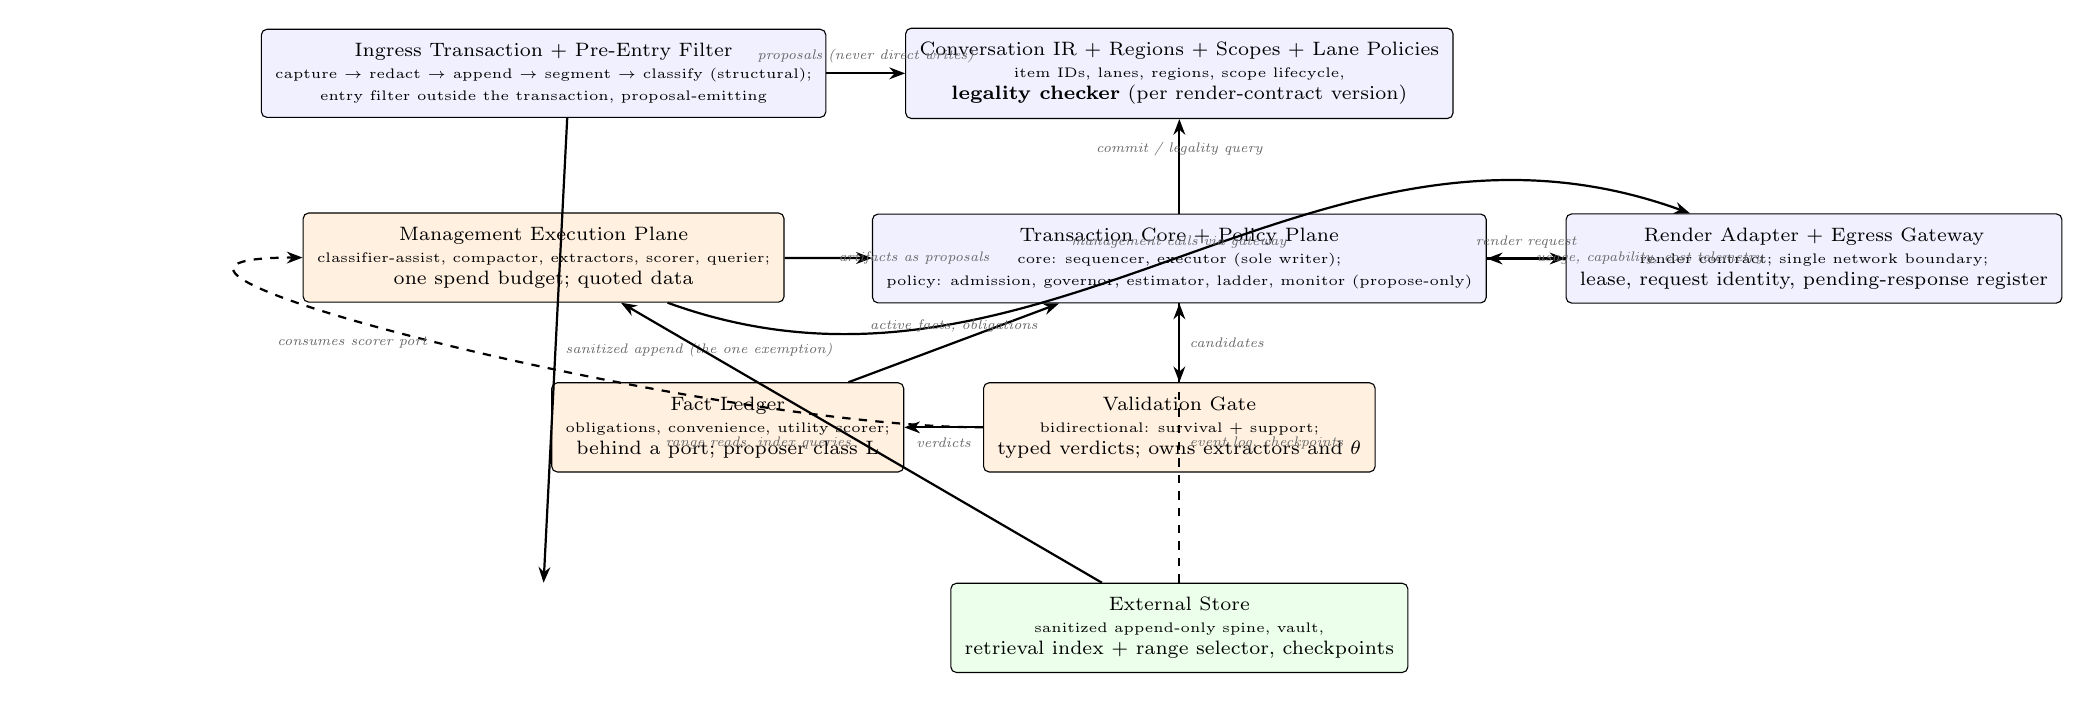
\begin{tikzpicture}[
  font=\scriptsize,
  box/.style={draw, rounded corners=2pt, align=center, inner sep=5pt},
  comp/.style={box, fill=blue!6},
  pol/.style={box, fill=orange!12},
  store/.style={box, fill=green!8},
  arr/.style={-{Stealth[length=2mm]}, thick},
  darr/.style={-{Stealth[length=2mm]}, thick, dashed},
  note/.style={font=\tiny\itshape, text=black!60}
]
\node[comp] (ing) {Ingress Transaction + Pre-Entry Filter\\ \tiny capture $\to$ redact $\to$ append $\to$ segment $\to$ classify (structural);\\ \tiny entry filter outside the transaction, proposal-emitting};
\node[comp, right=10mm of ing] (ir) {Conversation IR + Regions + Scopes + Lane Policies\\ \tiny item IDs, lanes, regions, scope lifecycle,\\ \textbf{legality checker} (per render-contract version)};
\node[comp, below=12mm of ir] (ctl) {Transaction Core + Policy Plane\\ \tiny core: sequencer, executor (sole writer);\\ \tiny policy: admission, governor, estimator, ladder, monitor (propose-only)};
\node[pol, below=12mm of ing] (mgmt) {Management Execution Plane\\ \tiny classifier-assist, compactor, extractors, scorer, querier;\\ one spend budget; quoted data};
\node[pol, below=10mm of ctl] (gate) {Validation Gate\\ \tiny bidirectional: survival + support;\\ typed verdicts; owns extractors and $\theta$};
\node[pol, left=10mm of gate] (ledger) {Fact Ledger\\ \tiny obligations, convenience, utility scorer;\\ behind a port; proposer class L};
\node[store, below=14mm of gate] (store) {External Store\\ \tiny sanitized append-only spine, vault,\\ retrieval index + range selector, checkpoints};
\node[comp, right=10mm of ctl] (mat) {Render Adapter + Egress Gateway\\ \tiny render contract; single network boundary;\\ lease, request identity, pending-response register};
\draw[arr] (ing) -- node[above, note] {proposals (never direct writes)} (ir);
\draw[arr] (ing.south) ++(3mm,0) -- node[right, note] {sanitized append (the one exemption)} (store.north -| ing.south);
\draw[arr] (mgmt) -- node[right, note] {artifacts as proposals} (ctl);
\draw[arr] (ctl) -- node[right, note] {candidates} (gate);
\draw[arr] (gate) -- node[below, note] {verdicts} (ledger);
\draw[arr] (ctl) -- node[above, note] {commit / legality query} (ir);
\draw[arr] (ctl) -- node[above, note] {render request} (mat);
\draw[arr] (mat) -- node[right, note] {usage, capability, cost telemetry} (ctl);
\draw[arr] (mgmt) to[out=-20,in=160] node[above, note] {management calls via gateway} (mat);
\draw[arr] (store) -- node[left, note] {range reads, index queries} (mgmt);
\draw[arr] (ledger) -- node[above, note] {active facts, obligations} (ctl);
\draw[darr] (store) -- node[right, note] {event log, checkpoints} (ctl);
\draw[darr] (gate) to[out=180,in=180] node[left, note] {consumes scorer port} (mgmt);
\end{tikzpicture}
}
\caption{Eleven boundaries (the diagram co-locates the ingress transaction with the pre-entry filter, the transaction core with the policy plane, and the render adapter with the egress gateway for layout). Solid arrows are committed data flow; dashed arrows are service dependencies. The untrusted writers, ingress, the management plane, and the policy plane, reach model-visible state only as proposals through the transaction core; the legality checker in the conversation IR is consumed by both the executor and the render adapter under a versioned render contract; the egress gateway carries every network request, conversation and management alike.}
\label{fig:arch}
\end{figure}

\section{Conversation IR, Region Model, and Scope Model}
\label{sec:ir}

Every incoming message (user input, tool result, model response) and every generated artifact (\S\ref{sec:derivation}) is segmented into items at a fixed pipeline stage; items cover the parent byte range totally and disjointly, checked at ingestion, and the composition with structure-preserving redaction keeps byte ranges stable across the redactor. Each item receives an immutable identifier at segmentation, a lane, and provenance: a versioned set of store ranges (not a single range), since a fold derives from multiple disjoint sources. Addressability survival holds at three declared levels: identifier resolution (always), metadata resolution (always), and payload availability (conditional on no erasure of the backing range; \S\ref{sec:store}).

\paragraph{Lane atomicity.} Lanes classify claims, and real messages mix claims: one user paragraph can carry a constraint, evidence, and exploration. In-transaction classification is structural and deterministic, so it cannot compute claim granularity; in-transaction lane assignment is therefore a conservative over-approximation, and the claim-granularity protocol runs as its own stage: when the structural classifier or the asynchronous refinement detects a lane-heterogeneous span, the item is split so that each item is claim-atomic, with byte provenance preserved across the split (the union of child ranges equals the parent range, checked at ingestion). Splits are performed by the logged resegment operation (Table~\ref{tab:ops}), which regenerates incompatible derivatives in the same transaction, so a mis-segmented item is repairable rather than permanent. For spans that cannot be split without destroying meaning (a failed attempt whose text embeds an exact error string), the precedence rule assigns the \emph{most-protective} applicable lane, and the entry filter still extracts the exact spans into the digest regardless of lane, so precedence never drops preserved evidence; protection-inflating over-approximations are a monitor signal, because they inflate the protected floor $M$ that the budget algebra must bound. Read-back answers and branch returns pass through the same protocol.

\paragraph{Regions.} The model-visible context is four regions over the IR: head (immutable constitutional content), near-head notes (the mutable ledger view; \S\ref{sec:ledger}), body (bounded folds whose granularity coarsens with age), tail (verbatim working set, floored). Regions are projections that partition \emph{placed} item references, not byte ranges: every durably admitted item is either placed in exactly one region or explicitly unplaced (store-only, reachable by read-back), duplication is suppressed at render, and occupancy is charged to the owning region. Extracting an item from a message for region placement preserves role legality by carrying a provenance tag the render adapter renders as a provider-legal message part. The mapping between the three protected-content notions is fixed: a lane is a property of an item; a region is a placement; a ledger entry is a fact that may or may not have a carrying item, and when it has none but is rendered through the notes view, its notes projection is the charged projection. The protection budget (\S\ref{sec:budget}) is computed over a union of item identities and charged projections, so no content is counted twice and no rendered fact is charged zero.

\paragraph{Scope model.} The IR boundary owns a scope registry, because five contracts read scopes (fold's closure precondition, declare-boundary, discharge, the gate's in-scope subset, branch isolation) and a convention without an owner is how silent corruption enters. A scope has an identifier stable across restarts (resolved from the log), lifecycle states (open, closed-by-event, closed-by-declaration) with the harness's scope events admitted as logged observations (scope-open, scope-close rows of Table~\ref{tab:ops}), nesting with item attribution (every item references the scope active at its ingestion, and child scopes attribute to their parent), and a defined fate on parent closure (open children remain open; their items are unaffected; only fold eligibility changes). Scope idleness, the precondition for declare-boundary, is evaluated over the log window (no items referencing the scope within the last $N$ log events), never over the tail projection, so reclamation cannot manufacture idleness.

\paragraph{Lane-policy registry.}
\label{sec:lanepolicy}
Typed retention is a registry, not a habit. The IR boundary owns a versioned registry that assigns each lane: a target fidelity (verbatim, field-preserving, digest, droppable), the permitted derivative operations, a droppability rank, and a survival-set class for the gate. Constitutional and decisional floors in the registry are safety-invariant parameters; evidential and ephemeral entries are profile-tunable (\S\ref{sec:params}). The preconditions of fold, compact, condense, and regenerate reference the registry version, and the gate selects survival sets by the registry's survival-set class, so the mechanism the compaction-cliff evidence motivates has one owner and one version \cite{cliff2026}. The ephemeral lane (superseded exploration, failed attempts) holds the first droppability rank, ahead of evidential: it is the cheapest semantic content to fold away and occupies the first rung of the reclamation ladder (\S\ref{sec:admission}).

\paragraph{Legality checker.} The boundary owns $\mathrm{is\_legal}(v, c) \to \mathrm{Result}\langle c, \mathrm{Violation} \rangle$ over a candidate version $v$ and a versioned render contract $c$ (the capability descriptor, profile, tool-declaration set, and serializer version the render adapter publishes as a logged value; \S\ref{sec:mat}), covering pairing integrity of calls and results, ordering, placeholder legality under $c$, per-region occupancy against budget, floors, pin protection, and the quoting convention of \S\ref{sec:threat}. $\mathrm{Violation}$ is enumerated (pairing, ordering, placeholder-illegal, region-over-budget, floor, pin, quoting-convention), each carrying the violated predicate, and the success type returns $c$'s version, so the executor and the render adapter can verify they evaluated the same contract rather than assuming it. The operation executor queries the checker before commit; the render adapter queries it before send. No other component decides legality, and legality depends on a data type rather than on the render adapter as a component, so the IR and the materializer side do not depend on each other.

\subsection{Derivation-Ingestion Contract}
\label{sec:derivation}
Generated artifacts are content like any other, and the contract is universal: \emph{any} content that enters a region without passing admit-ingress, which is to say every artifact of a model call (folds, compaction summaries, digests, branch returns, read-back answers, notes derived from generated text, promotions based on generated claims, repair-result markers, emergency-set synthesized markers, denial feedback rendered model-visible, imported content) re-enters through segmentation, classification, and redaction before admission, receives identifiers under the same scheme, and inherits lanes under the lane-partition rule. Derivation-ingestion is a synchronous sub-transaction of the owning operation, not a queued proposal: an in-flight operation completes its own artifact ingestion inline and never waits on the admission queue, whose service depends on that operation completing. This is a postcondition of the executor's \emph{generated} state. Without it, a compactor summary could copy a secret out of a quarantined range into head or notes without passing the redactor, because the three-artifact secrets model is an ingestion-plane mechanism; for the same reason, generated artifacts are volatile until derivation-ingestion completes, and the durable form of a \emph{generated} artifact is the sanitized artifact plus a vault reference (\S\ref{sec:txn}).

\section{Ingress Transaction and Pre-Entry Filter}

\paragraph{Ingress transaction.} Fixed order, ending at structural classification: volatile capture buffer, redactor (system authority, part of the transaction), sanitized append to the store (the one exemption), segmentation, structural classification. The transaction is synchronous, deterministic, and fail-closed; the pre-entry filter is deliberately outside it (\S\ref{sec:entryfilter}), so the security transaction's latency and correctness are never hostage to an evolvable rule registry. The capture buffer is volatile, bounded, ingestion-owned, and never persisted; a crash loses at most the un-redacted buffer, which is a declared loss. The store's ``raw'' events are post-redaction sanitized records; the document calls them sanitized sources for that reason. Classification inside the transaction is structural and deterministic (role, tool identity, pattern classes), so the transaction never blocks on a budgeted model call; model-assisted refinement runs asynchronously through the reclassify operation on structural results, and structural lane assignment is the documented fallback in Table~\ref{tab:consumers}. Recovery inside the transaction is deterministic for the same reason: if the sanitized append is durable but items are not, replay re-derives segmentation and structural lanes (deterministic); digests are produced outside the transaction and are pinned to rule versions, reproducible on replay.

\paragraph{Lanes as a partition.} Every item carries exactly one lane: constitutional (system prompt, task statement, explicit constraints, safety rules), decisional (commitments, verified state, open questions, standing decisions), evidential (tool outputs, file contents, logs), ephemeral (superseded exploration, failed attempts). The lane-partition rule of \S\ref{sec:ir} makes this a partition of claims rather than of messages. No derivative may carry authority its source lacked; this is a universal commit precondition with a check point (\S\ref{sec:invariants}).

\paragraph{Authority-sensitive admission grammar.} Obligation-pattern items (constraint-shaped, action-relevant content) are admitted to the ledger as obligations only from messages whose author authority is at least the agent's own (operator, user, agent-authored text). Environment-derived obligation candidates (a tool output containing TODO-like language) are quarantined as evidential until an authorized promotion; this closes the authority-laundering path into obligations. The decisional lane has its own laundering resistance, stated so that support and authority are checked as independent fields: a promotion of a derivative into decisional requires either a source item of same-or-higher authority or an authenticated adoption event by a principal authorized for that lane and scope; a gate pass establishes support and never substitutes for authority, so an agent following injected tool text cannot move it into the required-fact set by proposal or by citation. Ambiguous constraint-like content in operator or user messages is provisionally admitted flagged unconfirmed, within a bounded budget, and surfaces in validation. The authority lattice is operator over user over agent over environment, with scoped delegation; delegation binds to provenance, not file class: only configuration files named in the operator envelope or present and hash-pinned at session start carry delegated authority, since repository files are environment content an adversary can influence. Every proposal carries an authenticated principal.

\paragraph{Redactor contract.} The redactor declares detector classes (credential patterns, key material, token-shaped strings, declared-sensitive paths), a per-class recall posture with a stated target, structure-preserving replacement, and fail-closed behavior: on detector failure or timeout, the span routes to the encrypted vault and the sanitized record carries a vault reference rather than passing content through. Its residual (a missed class) is unrecoverable in an append-only store, so detector-class updates are operator-governed and the evaluation includes a leak corpus arm. Failure semantics appear in Table~\ref{tab:consumers}.

\paragraph{Pre-entry filter.}
\label{sec:entryfilter}
Rule-based, per-tool, over evidential items only, emitting proposals outside the ingress transaction. Each rule matches an output pattern and produces a preservation-aware digest with three declared classes of content: non-droppable exact spans (error strings, paths, line numbers, exit codes, test names, versions), ranked compressible content, and bulk noise. The guarantee is scoped honestly: every identifier class \emph{in the preservation vocabulary} that is detected in the raw observation appears in the digest; unrecognized strings are not claimed, and the residual (detected-but-dropped, in-class-but-undetected) is what the labeled-span preservation-recall arm measures (\S\ref{sec:eval}). Three conservatisms bound the residual: outputs below the size floor pass verbatim; an unknown-class span of unusual shape routes to the digest's verbatim section when its size is below a bound; and every digest carries the store raw handle, so nothing compressed at entry is unreachable later. Rules and the preservation vocabulary live in a versioned registry owned by the ingestion side; mutations go through the rule-update and vocabulary-update operations (Table~\ref{tab:ops}), and every historical version stays resolvable for the session's life because digests are durable artifacts pinned to the rule and vocabulary version that produced them. Rule updates split by direction: \emph{relaxation-only} changes (which can only preserve more) are permitted in-session, logged, rate-bounded, and reversible without offline qualification; \emph{tightening} changes require the offline qualification channel, because they can lose spans. Online rate control never works through rule tightening: sustained over-rate sources are handled by the governor's admission quotas and backpressure (\S\ref{sec:admission}), which preserves the relaxation-only invariant while still bounding admitted bytes. This preserves a bounded version of the intra-task adaptation TACO measured, while the offline channel governs the direction that can destroy evidence \cite{taco2026}. Ranking inputs (recency, error class, relation to ledger-active facts, defined in \S\ref{sec:ledger}) are declared as an open contract in \S\ref{sec:risks}; rule conflict resolution is by declared specificity order, with ties resolving toward the more preserving rule, and an unresolved tie is a declared rule error that fails the digest closed.

\section{Fact Ledger}
\label{sec:ledger}

The ledger is its own boundary behind a port with its own proposer class L, because domain state that constrains the agent must not live inside, or be mutated at the proposal of, the boundary that optimizes the agent's budget. The controller may request retirement with a budget justification; the ledger proposes and may refuse. The lifecycle operations (discharge, consolidate-obligations, demote, revalidate) are L-rows. It holds two classes. \emph{Obligations}: constraint-shaped, action-relevant facts admitted by the admit-obligation operation under the authority grammar above; they never decay, and they retire only through discharge, consolidate-obligations, or escalate (\S\ref{sec:ladder}). Discharge decisions run through a ledger-owned evaluator,
\[
\mathrm{discharge\_evidence}(\mathrm{obligation}, \mathrm{candidate}) \to \{\mathrm{resolved},\; \mathrm{superseded\;by},\; \mathrm{scope\_closed},\; \mathrm{insufficient}\},
\]
in which supersession and scope close are checkable from the ledger and the scope registry; resolution is checkable only through the gate, and an obligation counts as resolved only when the resolution claim is gate-supported to authenticated ingress spans; \emph{insufficient} is the default. \emph{Convenience memories}: admitted by admit-convenience under a utility scorer the ledger boundary owns, with contract $\mathrm{utility}(\mathrm{entry}) \to [0,1]$, comparable across entry ages under a declared normalization, computed from logged access and reuse events under calibrated weights, with the admission threshold a registered parameter (\S\ref{sec:params}); decay applies only here, through the logged decay operation. WMT motivates utility-weighted selection and measured memory poisoning; neither obligation retention nor poisoning resistance at this scale is validated by it, and both carry adversarial arms in \S\ref{sec:eval} \cite{wmt2026}.

Facts carry identity (subject, predicate, scope) and a two-axis status product: freshness (current, stale, unknown) $\times$ evidence status (verified, unverified), with the permitted transitions enumerated per operation (fact-invalidate: current $\to$ stale; redact: evidence $\to$ unverified; revalidate: stale $\to$ current only when the observation's read-set versions match; unknown $\to$ current never, without evidence). A fact is \emph{ledger-active} when it is an obligation or a convenience memory above the utility threshold, its freshness is current or stale, and it is not retired; this single definition is what the clear-class preconditions, the entry filter's ranking inputs, and the retrieval index's pinning rule all reference. \emph{Ledger-active} is defined here once. The supersession overlay is applied at commit time: an amendment rewrites the carrying fold in the same transaction, rather than rendering an overlay at request time, so deterministic re-materialization holds (\S\ref{sec:txn}). Depth increments only for semantic compaction, not supersession. Conflicts resolve by a deterministic matrix over two fact kinds: normative content (decisions, obligations) and empirical content (observations). Fresh tool evidence invalidates empirical premises whose read-set versions it supersedes; it never silently amends a normative fact, which changes only by an authorized amendment operation (amend, retract, escalate). A live decision resting on invalidated empirical premises surfaces as a flagged conflict to the model and the monitor, and is resolved by amendment, not by precedence. Freshness is tracked over declared invalidation dependencies from tool contracts, and invalidation is event-driven and atomic: when a tool result whose contract declares a write set is appended, the fact-invalidate operation transitions every in-domain current fact to stale in the same commit; revalidation consumes (observation, fact) pairs selected by read-set intersection, via the revalidate row, and the architecture runs no dedicated probes, which would contradict the no-re-execution boundary.

\section{Transaction Core and Policy Plane}

\subsection{Sequencer and Logical Time}
The sequencer assigns the total order and derives logical time (sequence numbers) for every policy predicate: queue aging, cooldowns, rate bounds, spend intervals, validity intervals, pin expiry, freshness over recorded elapsed time. Pin expiry is an explicit logged event proposed by the controller (expire-pin), not a passive transition, so replay reproduces it. Lease and fencing: every commit and every provider turn, conversation or management, carries the current epoch; a writer that observes a higher epoch aborts before applying, and the egress gateway (\S\ref{sec:mat}) suppresses late responses by request identity, so a superseded writer's model call cannot land. Fencing guarantees log integrity; fencing of world effects runs through the harness gateway with in-flight registration (\S2), and effects already dispatched are a declared residual no architecture can fence retroactively.

\subsection{Policy Plane: Admission, Governor, Monitor}
\label{sec:admission}
Queue classes with cross-class service: safety preemptions, ingress materialization, model proposals, controller economic triggers, monitor proposals, each with a reserved service share and a declared escalation rate, so a firehose of ingress cannot starve monitor proposals, which are the mechanism that relaxes over-aggressive filters. Queue service events are logged (queue-service row), so queue state is governed and replayable. Denials return bounded feedback naming an admissible alternative where the alternative-finding function finds one; its contract is $\mathrm{find\_admissible}(\mathrm{state}) \to \mathrm{List}\langle \mathrm{Op} \rangle$, a deterministic search over Table~\ref{tab:ops} in the table's fixed enumeration order with a bounded candidate set, owned by the policy plane and logged as an event so replay reads the recorded list rather than re-searching. The feedback text itself is system-authored content admitted through the admit-feedback row, with system authority and an explicit provenance tag, so it is governed content like any other. Re-proposals are deduplicated by semantic operation key (operation class, source ranges, source version), not by caller-provided identity, with a monotonic retry counter that ends in a different admissible operation or a terminal state; the rate limit applies to all re-proposals without exemption.

The \emph{ingress rate governor} bounds per-turn and per-window ingress bytes admitted into regions, and its backpressure contract is declarative and mechanical: a per-source, per-window admission quota whose exhaustion forces the handle path (admit-as-handle) regardless of size, plus declared producer backpressure; an observation that exceeds the per-round ceiling after entry filtering enters as a handle plus store pointer, never silently truncated. Filter rules are never tightened online (\S\ref{sec:entryfilter}). The governor's premise is enforced rather than assumed: the safety-invariant predicate $\mathrm{admitted\ rate} \le \alpha \times \mathrm{measured\ reclamation\ throughput}$ over the window, with $\alpha$ safety-invariant and the per-source quotas calibrated; on violation the governor tightens quotas to their floor, and if the predicate still fails, the declared quiesce transition follows (\S\ref{sec:budget}). The ingress-stress arm tests exactly this predicate (\S\ref{sec:eval}).

The \emph{runtime monitor} is a read-only observer over the event log, owned by the policy plane, emitting proposals under class C. Its signals are enumerated: repeated near-identical tool calls (reacquisition), re-read-after-reclaim clustering on one fold, requests for full output after a digest (over-compression), ladder-rung transition rate (thrash), and protection-inflating lane over-approximation (\S\ref{sec:ir}). Its proposals are read-back re-promotion, filter relaxation within the relaxation-only class, and escalations to the controller; it writes nothing directly. Sticky counters are controller-owned governed state incremented as a postcondition of re-promote, so on monitor failure the counters freeze (a logged, surfaced state) but no writer appears outside the transaction core.

The safety predicate uses dual thresholds (arm at $X$, disarm at $Y < X$) plus a reclaim target $T < Y$: any safety-tier intervention has the objective of reaching $T$, not merely crossing $Y$. Minimum inter-intervention spacing applies in disarmed and ordinary operation and is suspended while the safety tier is armed: safety reclamation is never blocked by spacing or by amortization economics. The arm and disarm transitions are themselves logged rows (arm, disarm). The trigger predicate is defined: project the materialized request size from current occupancy plus the measured per-round growth distribution over a recent window, and arm when the projection crosses $X$ before the next natural fold point; the growth distribution is governed state with contract $\mathrm{project\_growth}(\mathrm{window}) \to (\mathrm{distribution}, \mathrm{confidence})$, updated through the calibration-update class.

Selection is a constrained lexicographic ordering, the \emph{reclamation ladder}, whose fixed default order reclaims the middle before the tail and the cheap before the expensive: fold-away of ephemeral items (first droppability rank), placeholder-collapse of unpinned evidential body ranges (parameterized by region; on providers without placeholder tolerance this rung is skipped), fold, compact, condense (tail summarization at the last rung, under the stricter survival set that carries open questions and obligations verbatim). This ordering follows P8; condense exists because a floored-tail-only state leaves no cheaper rung. The selection-first prefix is a declared trade: generation provably dominates selection at equal error on some query families \cite{theory2026}, and the ladder accepts the weaker fidelity frontier for cost and determinism (no gate spend, no scorer dependency, available under scorer outage); the selection-first versus generation-first arm measures the trade (\S\ref{sec:eval}). The pressure estimator is a named policy-plane component with contract
\[
\mathrm{predict}(\mathrm{op}, \mathrm{range}, \mathrm{version}) \;\to\; (\mathrm{loss\_by\_lane},\; \mathrm{reclaim},\; \mathrm{invalidation\_cost},\; \mathrm{confidence} \in [0,1]);
\]
its state is durable and written only by the transaction core as logged operations; it is pure over (op, range, version, calibration-version); it may reorder only \emph{within} a rung of the fixed default order and never triggers ladder transitions, so the escalation index is always defined by the fixed order. Low confidence (threshold a registered parameter) falls back to the fixed default ordering. Cache cost enters selection two ways: every rewriting operation class carries an amortization-threshold precondition (expected invalidation cost below the operation's expected benefit, the generalized \texttt{clear\_at\_least} contract), suspended while the safety tier is armed, and invalidation\_cost breaks ties inside the estimator. Calibration runs through a declared offline channel (\S\ref{sec:eval}); its parameters belong to the calibrated governance class with bounds the loop may not exceed, so miscalibration degrades economic choices within bounded distance of the default and cannot touch safety-invariant parameters.

\subsection{Budget Algebra}
\label{sec:budget}
Conservation is stated over the materialized request in two layers. The enforced invariant, checkable locally, is
\[
\mathrm{bound}(v, c) \;\le\; B - R - H,
\]
where the token-accounting port has contract $\mathrm{bound}(v, c) \to \mathrm{Tokens}$ with declared properties: deterministic given $(v, c, \mathrm{margin\ version})$; additive over disjoint rendered content; conservative ($\mathrm{bound} \ge$ provider-reported tokens, the divergence band being the monitored obligation); comparable only within one render-contract version $c$. The materialization includes all request fields: region content, framing and role wrappers, tool declarations (an explicit tool-definition allocation $D$ that counts the context-management tool surface itself), placeholders and handles, and provider-added instructions under the capability contract. The provider-conditional obligation $\mathrm{tokens}(v) \le \mathrm{bound}(v)$ is monitored through the divergence band: divergence beyond the band recalibrates the margin (a logged operation) and tightens admission until they agree, and provider rejection is the declared violation handler. $B$ is the profile budget, $R$ the context reserve, $H$ the reserved output headroom.

Occupancy conservation and protection are \emph{universal commit preconditions}, not per-row notes: every commit that adds content anywhere must leave the post-state globally fitting $\mathrm{bound}(v', c) \le B - R - H$ and each region within budget, must preserve the protection budget, and must satisfy authority non-increase. The protection budget is stated in one unit over one set: let $M(v)$ be the bound of the \emph{minimum legal projection} of $v$ under the same render contract, computed as a union of item identities and charged projections (rendered constitutional items, obligations through their carrying items or notes projections, pinned bytes, tail floor, minimal valid scaffolding including role wrappers, pairing-critical records, and the full tool-declaration allocation $D$), each fixed request field counted exactly once. Protected content stays at or under $B - R - H$, feasibility is $M + R + H \le B$, and $M$ includes a \emph{terminal reserve} sized for the wrap-up prompt plus $H$, so the wrap-up branch is subject to fit like any row and can always render. Protection-checked admission covers the dominant growth source: obligations and constitutional content are admitted under the protection budget with a declared overflow policy (consolidate-obligations, the bounded unconfirmed queue, or explicit rejection surfaced to model and operator); constitutional ingress above the operator-set head budget is rejected at ingress by an explicit path. Pin admission additionally requires the reclaimability predicate: destination capacity for the atomic promotion is reserved (a safety-invariant fraction of the notes subregion that obligation admission may not consume) and the post-state protection budget holds, under aggregate and per-lane pin caps.

\emph{Net reclaim monotonicity.} One unit of account, the accounting port's conservative estimate over the entire post-state: every commit containing an operation of the \emph{reclamation class} (placeholder-collapse, drop-with-handle, fold, compact, condense, regenerate, demote, consolidate-obligations, consolidate-notes, pin-override-collapse; the rows credited as pressure relief) satisfies
\[
\Phi(v_{\mathrm{post}}) \;\le\; \Phi(v_{\mathrm{pre}}) - \mathrm{bar},
\]
evaluated at the executor's \emph{validated} state, where the minimum-reclamation bar is a safety-invariant parameter no profile may set to zero. Governance rows (redact, retract, discharge, escalate, quiesce) are outside the reclamation class: they carry their own authority and audit conditions and may grow occupancy, because their purpose is not pressure relief; semantic loss and budget reclamation are not overloaded. The earlier per-candidate form survives as a secondary provenance check only; the transaction-level inequality is what a note-then-fold or pin-override commit must satisfy \emph{net}. A candidate that fails the net bar routes to the next rung instead of committing.

\emph{Forward progress over the guarded transition relation.} Applicability is defined over the full precondition of each row, not over occupancy facts alone: capability class, scorer availability, cooldowns, spacing, pin state, the amortization threshold, and the net-reclaim inequality all gate applicability. While the safety tier is armed, the economic gates do not bind reclamation rows: spacing and amortization are suspended, and the estimator's reorder is bypassed in favor of the fixed order. $\Phi$ is comparable only within one render-contract version; a render-contract change (render-contract-observed, margin-recalibrate) is exempt from the freeze rule as an accounting-contract change, resets the measure, and if it makes the current state infeasible, forces the declared reclamation path immediately.

Let $\Phi(v)$ be the accounting-port estimate for version $v$ and $M(v)$ the protected floor as above. The active reclaim target is $T_{\mathrm{eff}} = \max(T, M)$. Progress is a case analysis over the region occupancy vector, stated per capability tier. In any feasible state with the safety tier armed, scorer available, and $\Phi > T_{\mathrm{eff}} + \mathrm{bar}$, at least one reclamation member applies, by cases: if the body contains ephemeral items, fold-away of ephemeral applies (semantic, cheapest); else if the body contains store-readable evidential items, placeholder-collapse over the body applies on placeholder-tolerant providers and drop-with-handle otherwise (deterministic); else if the body contains foldable scopes, fold applies; else if the tail is above floor, placeholder-collapse or drop-with-handle over the tail applies; else if pins exist and the reserved notes fraction has capacity, pin-override-collapse applies, reclaiming the non-pinned remainder of the collapsed range with the post-state floor bounded ($M' \le M +$ carried pinned bytes $\le T - \mathrm{bar}$), else routes to escalate; else if convenience memories are rendered, demotion applies with rendered reclaim at least bar; else if the body contains decisional derivatives, compact applies; else if the notes subregion contains non-obligation model-written notes, consolidate-notes applies (C-proposable within the recorded envelope; rendered reclaim at least bar); the residual case is an obligation-saturated floor, which is not a deadlock but the declared condition: the ladder routes to consolidate-obligations (rendered reclaim at least bar, bounded attempts), then to escalate within the unattended envelope or operator attention, then to the wrap-up branch. Under scorer outage or capability degradation, the same analysis holds over the deterministic member list (fold-away of ephemeral where precomputed derivatives exist, placeholder-collapse, drop-with-handle, demotion, convenience decay), and if no member applies, the residual is the \emph{quiesce} transition: a logged, surfaced, resumable terminal-declared state, never a silent no-op and never an unreachable path guarded by an unsatisfiable operation. The wall exists in the architecture only as the named branches (wrap-up, quiesce), each reached by a declared transition.

\emph{Termination and stability.} The claim is stated over macrosteps, not over every commit. A macrostep is one armed intervention episode ending in a reclamation commit. Let $\Psi = \Phi + q$, where $q$ is queued mandatory ingress measured in accounting-port units, and let $r^-$ be retries remaining. Under the enforced governor predicate (admitted ingress rate $\le \alpha \times$ measured reclamation throughput, \S\ref{sec:admission}), every macrostep decreases $(\Psi, r^-)$ lexicographically: reclamation commits decrease $\Phi$ by at least bar, mandatory-ingress commits between interventions decrease $q$ without raising $\Phi$ past the governor bound, and failed attempts consume $r^-$ without changing $\Phi$. Two theorems are claimed, both conditional on the governor predicate, which is enforced and stress-tested rather than assumed: \emph{stability}, under continuing bounded ingress with the predicate holding, $\Phi$ remains within $[M, X + \delta]$ for a bounded overshoot $\delta$; and \emph{termination}, once ingress closes or the governor quiesces it, armed episodes end in a disarmed state, wrap-up, or quiesce within bounded macrosteps. A rate inequality is an amortized throughput property and is claimed as exactly that. Content-adding actions in disarmed states raise $\Phi$ freely; that is what the arm threshold is for.

\subsection{Operation Executor}
\label{sec:executor}
Operations run a durable state machine (proposed, snapshotted, generated, validated, committed, aborted). Artifacts become durable at \emph{generated} in sanitized form (\S\ref{sec:derivation}); gate verdicts at \emph{validated}. Every operation carries an identity and names its parent version; the commit is a compare-and-commit: if the current version is not the named parent, rebase-safe classes (note, read-back under the governor) re-apply against the actual parent, and all others abort and re-propose with fit, legality, protection, and required-fact extraction re-evaluated against the actual parent. The commit event is the atomic unit: region swap plus ledger events plus index updates plus checkpoint hooks commit together or not at all; replay is the deterministic reducer over the unique, deduplicated event sequence. Universal commit preconditions (fit, protection, legality, authority non-increase, net reclaim for the reclamation class) are enforced by the executor for every row, so no row can omit them by accident. The closure sentence reads: every mutation of the derived governed-state enumeration of \S4 is one of the operations in Table~\ref{tab:ops} (proposer classes S system, C controller, M model, O operator, U user, L ledger), and every deterministic system transition is itself an enumerated row; rows that constrain the model additionally require the named principal predicate, so the agent under budget pressure cannot retire the facts that constrain it. The conformance program re-derives the enumeration from the table and fails on any governed event type with no row.

\subsection{Degradation Ladders}
\label{sec:ladder}
Two ladders with declared precedence over each other: the \emph{reclamation ladder} is the outer loop and owns rung selection (\S\ref{sec:admission}); the \emph{escalation ladder} is bounded to a fixed retry count \emph{within} a rung, and on exhaustion returns control to the reclamation ladder at the \emph{next} rung in the fixed default order, never to lower aggressiveness in the same rung, so the two cannot oscillate (escalate aggressiveness, fail the gate, lower aggressiveness, lose the net bar, escalate again). Total retries per pressure event are bounded and counted as a metric. The escalation ladder answers gate and provider failure, split by verdict class: completeness failures retry at lower aggressiveness (an operation parameter: target ratio for compact, granularity for fold, declared in each contract), then narrower scope, then abort to the next rung; precision failures regenerate with the offending assertions excluded, then abort; provenance failures abort immediately and never retry. The escalation ladder also answers provider rejection or an armed safety tier, and escalates reclamation monotonically along the fixed order: admitted operation at the current rung under the capability-adjusted ladder (on providers without placeholder tolerance, drop-with-handle is an ordinary rung, not an emergency member), then the deterministic emergency set, then declared degrade via escalate (authorized, logged, surfaced obligation retirement; the operator envelope maps to controller-exercisable bounds recorded before the run) as a two-phase transition (escalate-pending blocks further escalation and retires nothing; escalate-complete performs the separately validated mutation), then the wrap-up branch (a minimum-safe-budget conclusion preserving store, ledger, and a resumable checkpoint), and, when even wrap-up cannot render because the terminal reserve has been consumed by protected content, the quiesce-unwritable path (\S\ref{sec:store}).

The emergency set is an enumerated subset of ordinary operations flagged deterministic, each a row of Table~\ref{tab:ops} with computable maximum serialized size before invocation: placeholder-collapse of unpinned evidential items; logged pin-override-collapse (the non-pinned remainder reclaimed, pinned bytes carried verbatim into the reserved notes fraction within the protection budget, else inadmissible and the state routes to escalate); drop-with-handle over tail or body with a synthesized textual marker legal in a plain message list; convenience demotion. When the scorer is unavailable and semantic operations fail closed, these members still reclaim without a gate, because they are deterministic and carry only store-readable or verbatim-carried content.

\section{Operation Set}
\label{sec:ops}

Table~\ref{tab:ops} is the closed set. Proposer is who may propose; authority names the required principal where it exceeds the proposer's. Model-callable rows are propose-only: the transaction core schedules. The model-facing tool surface is exactly the set of M-rows (note, read-back, pin, unpin, promote, amend, retract, reclassify, reopen, branch-open, branch-return, branch-abort, rule-update, vocabulary-update within the relaxation-only class); its declarations are counted inside $D$, and denials reach the model as governed tool-result content (\S\ref{sec:admission}).

{\footnotesize
\begin{longtable}{@{}p{2.35cm}p{1.15cm}p{4.6cm}p{5.6cm}@{}}
\caption{Closed operation set. S system, C controller, M model, O operator, U user, L ledger (proposer); universal commit preconditions (fit, protection, legality, authority non-increase, net reclaim for the reclamation class) apply to every row and are not repeated. The governed-state enumeration of \S4 is re-derived from this table's precondition and postcondition columns.}\label{tab:ops}\\
\toprule
\textbf{Operation} & \textbf{Proposer} & \textbf{Preconditions} & \textbf{Postconditions and guarantees} \\
\midrule
\endfirsthead
\toprule
\textbf{Operation} & \textbf{Proposer} & \textbf{Preconditions} & \textbf{Postconditions and guarantees} \\
\midrule
\endhead
admit-ingress & S & ingress transaction complete & sanitized append durable; segmented items, structural lanes durable; unplaced (store-only) until a placement commits \\
admit-observation & S & admit-ingress done; governor quota satisfied or handle path taken & item placed in tail region; pairing integrity preserved; post-state fits \\
admit-as-handle & S & observation exceeds ceiling after filtering or quota exhausted & handle plus store pointer in tail; raw reachable; pairing preserved \\
admit-feedback & S & denial feedback synthesized & system-authored content with system authority and explicit provenance tag; governed like any content \\
pending-response-stage & S & provider response arrived & response held in non-model-visible register bounded by pre-send output allowance; freeze-exempt into the register only \\
admit-response & S & pending register nonempty & atomic reclaim-or-handle transaction places response and per-call execution-intents; overflow routes to handle path dropping reasoning first; post-state fits \\
admit-obligation & S & authority grammar pass; protection budget holds or overflow policy invoked & obligation durable; overflow routes to consolidate / unconfirmed queue / rejection (logged) \\
admit-convenience & S & utility score above registered threshold; ledger bound not reached & convenience memory durable; decay-eligible \\
sanitize & S & detection at ingress & part of ingress transaction; structure-preserving; per-class recall posture; fail-closed to vault \\
redact & O & retroactive request; dependent check passes & crypto-erasure of vault material plus tombstone; dependents render as tombstones; pre-erasure hashes become unverifiable by design (logged cause); post-erasure checkpoint issued; facts move to unverified \\
note & M/C & precision-direction gate pass; priced at prefix cost; envelope rate bound & durable and flushed before any lossy op on source (flush-notes); structurally non-supporting: never a support leaf for other generated assertions \\
read-back & M & query within retrieval budget (coupled to safety-tier state); post-state fits & deterministic range and pagination reads as baseline; query path lane-pinned; answer enters via derivation-ingestion \\
re-promote & C & monitor signal; sticky counter below cap & targeted re-injection of a recently reclaimed range; controller-owned counter increments \\
placeholder-collapse & C & region parameter (body or tail); unpinned evidential items; provider tolerates placeholders & deterministic; placeholder retained with call record; net reclaim at least bar \\
drop-with-handle & C & target range store-readable evidential (tail or body) & deterministic; handle plus synthesized marker; net reclaim at least bar \\
fold-away-ephemeral & C & ephemeral items in body & semantic fold of ephemeral lane to store-only; net reclaim at least bar; cheapest rung \\
condense & C & tail above floor; last-rung position; stricter survival set; protecting notes flushed and rendered; post-state fits & replaces the tail projection atomically; per-lane partition derivatives per lane-policy registry; obligations verbatim or note-promoted first; net reclaim at least bar \\
fold & C & scope closed (event or declared boundary); lane-policy registry version referenced; obligations verbatim or note-promoted first (flushed); post-state fits & per-lane derivatives; provenance retained; net reclaim at least bar; note-then-fold atomic \\
compact & C & body at size cap or boundary event (projection crossed $X$ with cooldown elapsed, or wrap-up trigger) & per-lane summary chain per lane-policy registry; provenance fields retained; post-state fits; net reclaim at least bar \\
regenerate & C & body at depth cap & bounded, lane-typed input selection re-read from store ranges; depth reset; gate pass required; net reclaim at least bar \\
pin-override-collapse & C & pins present; reserved notes fraction has capacity; non-pinned remainder reclaim at least bar; post-state $M$ bound holds & non-pinned remainder reclaimed; pinned bytes carried verbatim into notes; logged override; else routes to escalate \\
demote & L & rendered convenience memories present; rendered reclaim at least bar & ledger and rendered relief; never obligations \\
discharge & L & discharge\_evidence returns a verdict other than insufficient (resolution gate-supported) & obligation retirement (one of three paths); insufficient is the default and retires nothing \\
consolidate-obligations & L & obligation set overflow or protection floor above $T - \mathrm{bar}$; rendered reclaim at least bar; attempt counter below bound & validated merge to same-or-higher-authority composite; union of bindings; surfaced; exhaustion routes to escalate \\
escalate-pending / escalate-complete & O (or C within recorded envelope bounds) & emergency set exhausted; logged surfacing & pending blocks further escalation and retires nothing; complete performs the separately validated mutation after surfaced retirement \\
amend / retract & M & principal same-or-higher than original; non-obligation entries only & commit-time supersession rewrite; no render-time overlay \\
promote & M & target-lane principal: same-or-higher authority source, or authenticated adoption event by an authorized principal (gate pass is support, never authority) & lane change; occupancy fit; support and authority recorded as independent fields \\
reclassify & M & evidence contract: operator assertion, classifier-assist (protection-decreasing only), or monitor signal plus versioned policy; into decisional or constitutional requires the promote predicate & atomic regeneration of incompatible derivatives in the same transaction \\
resegment & M/C & monitor signal or classifier-assist; claim-atomic re-split computable & child ranges union to parent; incompatible derivatives regenerated atomically; logged \\
reopen & M & post-state fits; bounded like read-back & recalled range re-enters via derivation-ingestion; provenance recorded \\
pin & M & reclaimability predicate holds; caps and protection budget hold & range protected from placeholder-collapse, condense, fold \\
unpin & M & principal owns the pin, or explicitly higher authorized principal within scope; target resolution is a separate existence precondition & protection released; expire-pin is the sole non-owner release path \\
expire-pin & S & logical-time window elapsed & logged event; protection released \\
declare-boundary & C & no harness scope event within aging window; scope idle over the log window & synthetic boundary recorded; folds at it use the stricter survival set \\
scope-open / scope-close & S & harness scope event observed & lifecycle state change in the scope registry; fold eligibility updated; logged \\
decay & S & decay interval elapsed in logical time; convenience class only & logged utility decay; no other class \\
flush-notes & S/C & flush-epoch boundary and amortization bar satisfied, or forced-flush trigger (lossy op waiting on a noted source; armed tier, priced unamortized) & batched note writes become rendered; gate completeness is evaluated on the rendered post-state \\
arm / disarm & S & projection crossed $X$ (resp.\ fell below $Y$); minimum spacing (suspended while armed) & safety-tier state change; logged \\
rule-update & M/C & relaxation-only class: rate bound, logged, reversible; tightening: offline qualification recorded & new rule version durable; all prior versions resolvable \\
vocabulary-update & M/C & as rule-update & as rule-update \\
fact-invalidate & S & tool result with declared write set appended & in-domain current facts transition to stale, atomically with the result append \\
revalidate & L & (observation, fact) pair selected by read-set intersection; observation read-set versions match & stale $\to$ current only on version match; else no transition (deterministic fallback) \\
stale-demote & S & resume event (new observation arrived in a domain holding stale facts; sequencer vocabulary) & logged; evidence-status change on stale facts \\
repair-result & S & recovery found an unpaired call, with or without a prior intent record & synthesizes indeterminate tool result; IR legality restored; side-effect rule keyed on the harness intent record \\
branch-open & M & constitutional replication; budgets inherited; depth and concurrency caps; read-only tool class only & namespace-isolated subtrajectory with ledger read view \\
branch-return & M & parent version unchanged, or conflict path (parent write intersects branch read set) taken; gate verdict pass & result enters via derivation-ingestion; carries no authority; conflicted returns admitted as evidential suggestions with ledger revalidation \\
branch-abort & M/C & branch drifts out of scope, exceeds spend, or is abandoned & slot released; partial store rounds retained; no return content \\
checkpoint & S & internal trigger (event count, byte volume, commit count) & bounded replay point durable; later log entries replayed, never discarded \\
lease-acquire & S & epoch monotonic; in-flight executions drained or marked indeterminate & single-writer epoch established \\
render-contract-observed & S & render adapter published a new render-contract input (capability descriptor, profile, tool declarations, serializer, tokenizer) & versioned input logged; request hash scope moves with it; measure comparability resets; infeasibility forces the reclamation path \\
calibration-update & S & offline channel verdict; within class bounds & estimator weights, decay weights, growth distribution, margin updated; logged \\
margin-recalibrate & S & divergence band exceeded & over-estimate margin updated; admission tightened until agreement; logged \\
store-mode & S & capacity admission or durability observation & read-only / unavailable transitions; quiesce contract armed \\
queue-service & S & queue class service event & accounting durable; queue state governed and replayable \\
spend-account / journal-append & S & spend event or rewrite event & accounting and rewrite journal durable (core-written logged events) \\
wrap-up & C & infeasibility branch or envelope exhaustion; terminal reserve renders; store writable & minimum-safe-budget conclusion; store, ledger, checkpoint preserved; terminal; subject to fit like any row \\
quiesce-unwritable & S & storage unavailable or terminal reserve consumed & write-free path; out-of-band operator output; no committed terminal state claimed \\
index-rebuild & S/O & recovery or operator request & retrieval index rebuilt from sanitized records \\
import & O & operator trust decision & routed through redactor and segmenter; admitted as evidential with provenance \\
consolidate-head & O (or C within recorded envelope bounds) & near-head notes overflow; operator or preauthorized policy & notes subregion rewritten under validated summary; constitutional items never rewritten, only retired by operator-approved replacement with exact rule preservation; surfaced \\
consolidate-notes & C & notes subregion saturated with non-obligation notes; within envelope; rendered reclaim at least bar & bounded consolidation of model-written notes; surfaced \\
\bottomrule
\end{longtable}
}

\subsection{Branch Construct}
\label{sec:branch}
A branch runs a token-heavy exploration as an isolated subtrajectory whose rounds enter the store but never the working context \cite{folding2026,dream2026}. The spawn contract records parent version, dependency projection from notes, both budgets (context and management spend), depth and concurrency bounds, a namespace, and the tool-class restriction: branches run read-only tool classes only. Side-effecting branches are out of scope, declared as a dependency on the harness's own concurrency control (\S2), because transcript isolation does not isolate a shared filesystem and conflict-checked serialization of world effects is harness machinery, not context management. The return carries an environment-version check derived from the \emph{read sets} of the tools the branch executed: if a parent write intersects a branch read set, the conflict path admits the return as an evidential suggestion with ledger revalidation rather than as a current result. Constitutional replication into every branch context is a precondition of branch-open and a checked postcondition: partitions that do not replicate scoped rules produced 93\% locality violations in topic-partitioned memory against 0\% with replication, and the transfer of that mechanism to branch contexts is labeled as such \cite{cliff2026}. The return is admitted through the derivation-ingestion contract, passes the gate, and carries no authority. Branch storms are bounded by the concurrency and depth caps, by spend allotment, and by branch-abort, which releases slots so abandonment (the dead-end reset AgentFold motivates) cannot leak them into an admission deadlock \cite{agentfold2026}.

\section{Validation Gate}
\label{sec:gate}

The gate is an oracle: verdicts in, nothing else. Its verdict type is closed and typed by failure class:
\[
\begin{aligned}
&\mathrm{validate}(\mathrm{candidate}, \mathrm{leaves}, \mathrm{required\_facts}, \theta) \;\to\\
&\quad\{\,\mathrm{pass},\; \mathrm{fail\_completeness}(\mathrm{missing}),\;
\mathrm{fail\_precision}(\mathrm{unsupported}),\\
&\qquad\; \mathrm{fail\_provenance}(\mathrm{cycle} \mid \mathrm{ungrounded\_root})\,\},
\end{aligned}
\]
and the escalation ladder's response is a function of the class (\S\ref{sec:ladder}). It owns three internal components, declared and funded as management-plane consumers (Table~\ref{tab:consumers}): the required-fact extractor, the assertion extractor, and the entailment scorer port (the scorer runs in the management plane, but the port, the prompt, the independence requirements, and the threshold $\theta$ are gate-owned, which keeps validation independence from the compactor a structural property the error-correlation arm measures rather than an assertion). The extractors have declared mechanism classes and fallbacks: required-fact extraction falls back to the deterministic union of ledger obligations plus constitutional items plus declared pattern classes; assertion extraction has no semantic fallback and the gate fails closed on its failure.

It is bidirectional. \emph{Completeness}: the required-fact set (constitutional items, obligations, decisional items in scope, selected by survival-set class from the lane-policy registry) must be recoverable from the \emph{rendered} post-operation context, with binding-aware checks, meaning an exact string survives with its qualifier context (command, negation, scope, temporal marker) and relation fields are checked as tuples, not byte presence; evaluation on the rendered post-state is what makes a durable-but-unrendered note insufficient, and flush-notes is a precondition of any lossy commit that waits on a noted source. Survival sets are typed per content class following the typed-retention result, with the transfer from knowledge-base triage to coding-agent facts labeled a hypothesis \cite{cliff2026}. \emph{Precision}: every assertion in a generated artifact must carry extractive or entailment support, and support is rooted in \emph{authenticated ingress leaves}: each generated assertion is scored directly against a bounded set of leaves, where a leaf is a sanitized source span appended by admit-ingress together with its authenticated principal metadata. Generated intermediates carry provenance pointers for navigation, but they are never entailment evidence; a validator error therefore cannot propagate, because a false acceptance cannot serve as support for the next round. When summaries are compacted repeatedly, the leaf set is carried forward under a declared cap and refreshed from store ranges when the cap binds; the residual risk that a capped leaf set drops a needed leaf is recorded in \S\ref{sec:risks}. Cycles among pointers are rejected as provenance failures. Contradiction checks run over the in-scope subset plus an always-checked class (constitutional and obligation facts), priced in the management spend budget. The semantic threshold $\theta$ is safety-invariant. False acceptance in the release-blocking benchmark sense is a stop condition for release, with the gate's own precision and recall measured against a labeled corpus before release, and offline tuning of compression quality uses paired closed-loop continuations \cite{trace2026}.

\section{Management Execution Plane}

Six consumers (classifier assist, compactor, required-fact extractor, assertion extractor, entailment scorer, read-back querier) run behind this boundary under one spend budget, separate from the context reserve. Inputs are enveloped as quoted data under an instruction preamble; outputs are data until a promotion operation with an authorized actor makes them otherwise, and derivatives never carry authority. Quoted-data envelopes plus authority metadata make management-call injection a formal non-elevation; they do not by themselves stop the task model from following instructions embedded in tool output, which is why the threat model (\S\ref{sec:threat}) specifies task-model serialization isolation and records the residual risk. Each consumer has declared failure semantics (Table~\ref{tab:consumers}); the spend budget reserves a safety share with a gate-only sub-share no other consumer may draw from, sized so that extraction plus scoring of every candidate the compactor can produce under the remaining share fits, because a gate starved by the compactor fails closed into the emergency set at precisely the wrong moment. The spend budget replenishes per provider turn (a declared logical-time interval); when exhausted, non-safety consumers queue and the deterministic fallbacks of Table~\ref{tab:consumers} carry the load.

Every management call is a network request and therefore follows the provider-turn protocol through the egress gateway (\S\ref{sec:txn}): durable call-intent with request identity before send, at-most-one-attempt per identity for non-idempotent classes, late-response suppression, spend charged at intent, fencing by epoch. Management calls do not pass the legality checker or the conversation render path; they pass the gateway, the accounting port, and the telemetry port, which is the same contract the failure table and the cost ledger rely on.

{\footnotesize
\begin{longtable}{@{}p{2.6cm}p{3.6cm}p{3.8cm}p{3.5cm}@{}}
\caption{Per-consumer and redactor failure semantics.}\label{tab:consumers}\\
\toprule
\textbf{Consumer} & \textbf{On failure} & \textbf{Deterministic fallback} & \textbf{Effect on operations} \\
\midrule
\endfirsthead
\toprule
\textbf{Consumer} & \textbf{On failure} & \textbf{Deterministic fallback} & \textbf{Effect on operations} \\
\midrule
\endhead
classifier-assist & refinement unavailable & structural lane assignment (in-transaction default) & weaker lanes, bounded by promotion-only decisional \\
compactor & condense, fold, compact, regenerate unavailable & emergency set & reclamation ladder skips semantic rungs \\
required-fact extractor & model-assisted refinement unavailable & deterministic union of obligations, constitutional items, pattern classes & completeness check coarsens, never silently passes \\
assertion extractor & failure & none: gate fails closed & no semantic replacement of live context \\
entailment scorer & gate fails closed & emergency set & no semantic replacement of live context \\
read-back querier & query path down & deterministic range and pagination reads & F3 risk rises; surfaced \\
redactor & detector failure or timeout & fail-closed to vault, reference in sanitized record & nothing unscanned reaches the store \\
monitor & signal source down & signals stop; no proposals; counters frozen (logged) & relaxation and re-promotion pause; surfaced \\
spend exhausted & non-safety consumers queue & safety and gate-only shares reserved & safety-tier reclamation, extraction, and gate continue \\
\bottomrule
\end{longtable}
}

\section{External Store}
\label{sec:store}

The store is append-only over sanitized records and never shrinks, and losslessness is stated precisely: after an ingress commit, the sanitized record is byte-preserving and durable, and every live item resolves to store ranges at the identifier and metadata levels; before the commit, the volatile capture buffer is a declared loss; payload availability is conditional on erasure. The secrets model spans three artifacts with one owner each: the capture buffer (ingestion-owned, never persisted), the sanitized record and the encrypted vault for material the redactor quarantines (store-side). The redact operation carries a dependent check so dependents of erased material render as tombstones with status markers and their facts move to unverified. The retrieval index and range selector live on the store side behind a port the management plane consumes: deterministic identifier and range reads with pagination form the baseline; query retrieval ranks with lane-typed pinning ahead of relevance, so constitutional and ledger-active content (defined in \S\ref{sec:ledger}) is always in the candidate set \cite{cliff2026}. Store capacity has an admission contract with enumerated mode transitions (store-mode row: normal, read-only, unavailable): read-only admits reads and quiesces writes; unavailable quiesces everything. When durability is unavailable, no state-advancing turns and no side-effecting tool executions occur, and the session quiesces in place through the write-free quiesce-unwritable path, which produces out-of-band operator output and claims no new committed state; a durable wrap-up is a different row, admissible only while the store is writable. Checkpoints bound replay without discarding later durable entries: recovery replays the log tail after the last checkpoint, and a corrupt tail is surfaced as an integrity failure, never silently truncated.

\section{Render Adapter, Egress Gateway, and Provider Capability Contract}
\label{sec:mat}

Two components behind one section. The \emph{render adapter} renders the IR into provider requests through the legality checker (it does not own legality; it publishes the render contract) and owns the conversation-specific capability contract: placeholder tolerance (absent: drop-with-handle is an ordinary rung), prefix-stability classes, tool-declaration accounting, tokenizer availability, and provider-added-instruction accounting. Capability and render-contract descriptors are versioned values: the render-contract-observed operation logs a new version for any input change (capability descriptor, profile, tool declarations, serializer, tokenizer), and the request hash and the legality checker's parameterization are scoped to that version, so provider-side drift is a logged event with a defined recovery rule (re-render under the new contract, forced reclamation if infeasible) rather than a silent integrity failure. The \emph{egress gateway} is universal and conversation-independent: it enforces the lease at send admission, carries request identity, suppresses late responses, holds the pending-response register, and implements the token-accounting and telemetry ports both the conversation path and the management plane consume. Management calls take the gateway, the accounting port, and the telemetry port, never the render path. The controller never reaches into either component; policy depends on the ports.

The gateway enforces the lease at send admission: a request is admitted to the network only if its epoch is current, and late responses are suppressed by request identity, for conversation and management calls alike. $H$ is enforced as a request parameter (max output tokens) where the provider supports it, and the pending-response register is bounded by the pre-send allowance; a response larger than the register routes through the overflow path (handle plus digest, reasoning dropped first), the provider context-editing precedent adapted \cite{anthropic2026docs}. Provider classes carry per-class delivery semantics and support postures: stateless attested providers get the full restart-equivalence guarantee; providers with idempotent request identities or an attested status query get at-most-one-send knowledge; providers without idempotency get at-most-one-\emph{attempt} per identity, and any send-intent unresolved at recovery is marked indeterminate and never resent, because the durable state cannot distinguish crash-before-send from crash-after-send and only the original live process may move from durable intent to send; stateful or unattested providers are excluded from restart-equivalence claims, their conversation state is treated as unobservable, and unattended runs refuse them outright.

\section{Transactional Semantics}
\label{sec:txn}

Deterministic re-materialization is an invariant with a scoped statement: rendering the log prefix through committed version $v$ \emph{under the render-contract version recorded with $v$} is a pure function for every version whose backing payloads remain available, and every render dependency (profile, capability descriptor, tool declarations, serializer and tokenizer version, over-estimate margin) is a versioned, logged input (render-contract-observed, calibration-update, margin-recalibrate). After an erasure, rendering is defined as the latest erasure-overlay view; hashes of pre-erasure versions become unverifiable by design (the logged redaction is the cause), and a post-erasure checkpoint and hash are issued. The store records a content-addressed hash of each materialized request scoped to its render-contract version; recovery verifies hash equality, a mismatch with a logged cause (redact, render-contract change) is expected invalidation, and a mismatch with no logged cause is an integrity failure surfaced, never silently re-derived. Commit-time supersession rewrites, durable digests pinned to rule versions, and flush-epoch-batched note commits are the mechanisms that make purity hold.

The provider-turn protocol, uniform for conversation and management calls: a durable send-intent carrying the request identity and hash is written before send; the committed context version and the request hash are durable before send; the response arrives into the pending-response register (bounded by the pre-send output allowance, freeze-exempt as a register write, not as a region write); admit-response then consumes the register through one atomic reclaim-or-handle transaction that places the response and its per-call execution-intents or routes the overflow to the handle path, so a normal response always has a legal commit and a $\Phi$-increasing arrival never violates the freeze rule, because the admission is net-nonpositive by construction. A durable per-call completion record follows each tool execution, keyed on the harness intent record. Recovery rules by interval: before send-intent, nothing happened; after send-intent unresolved at recovery, the intent is marked indeterminate and never resent (non-idempotent classes), or retried with the same identity where the provider class allows idempotency or an attested status query; after the atomic response-plus-intent append without a completion record, side-effecting tools are never re-executed and repair-result synthesizes an indeterminate tool result so the IR stays legal, with the side-effect rule keyed on the intent record (no intent record for a call means no side effect occurred, so the call may be scheduled or the response discarded under a declared rule); tools declared idempotent may re-execute per their harness contract; mid-execution, the same rule applies to the un-executed remainder. Crash intervals for management calls are the same protocol on the call-intent record, with the artifact pipeline adding one rule: generated output is volatile until derivation-ingestion completes, so a crash between generation and sanitization discards the artifact and re-proposes the operation (deterministic members are unaffected); the durable \emph{generated} artifact is the sanitized text plus a vault reference, which is what replay resumes from. Ingress is one transaction (sanitize, append, segment, classify structurally) whose visible result is all-or-nothing, with the deterministic recovery rule of \S6 and the entry filter re-proposing outside it. Idempotence-under-replay is a postcondition of every committed operation, realized through operation identities, semantic dedup keys, event uniqueness, and the deterministic reducer.

\section{Cache Economics}

A rewrite journal (the word ledger stays reserved for the fact ledger) records every prefix-rewriting event with tokens reclaimed, invalidation cost priced from telemetry when it exists, and logical time plus recorded wall time since the last rewrite. Head and note writes are priced in selection at full-prefix invalidation cost through the amortization-threshold precondition and the estimator's invalidation-cost term; note writes are committed in batches at flush-epoch boundaries (a distinct notion from the fencing epoch) with a declared amortization bar, and a forced flush is a \emph{precondition} of any lossy commit waiting on a noted source, priced separately and honestly as an unamortized write; while the safety tier is armed, amortization is suspended and every note-flush is unamortized, a sustained-armed cost the metrics report rather than hide. The alternative placement (notes after body) trades P8 for prefix stability and is rejected as a default pending measurement, with a notes-placement ablation in \S\ref{sec:eval}. The controller prefers operations that append (branching, noting at flush-epoch boundaries) over operations that rewrite.

\section{Multi-Day Continuity}

A multi-day task is a chain of bounded windows over one store. On restart or reset, the head reconstructs from constitutional content plus durable notes, the body from the latest validated compaction state, and the tail from recent store rounds; stale-demote runs as a logged operation; the model operates under a standing instruction that anything not written to notes is at risk, which is the memory-tool protocol prompt adopted as architecture \cite{anthropic2026cookbook}. Unattended operation is a first-class mode: the operator envelope pre-authorizes consolidation policy, escalation bounds (which the escalate rows exercise as controller-checkable limits), and the delegated-configuration allowlist; constitutional admission at ingress is bounded by an operator-set head budget with an explicit rejection path; and verified-state tracking (done, checked, remaining, each claim citing store provenance) lives in the decisional lane and notes, answering the calibrated-stopping failure LHTB documents \cite{lhtb2026}. The guarantee is stated precisely: bounded continuation while the minimum-safe projection fits, followed by controlled termination through the declared branches. Whether protected-content growth stays within that bound over days is an empirical question the endurance protocol measures; the architecture does not claim indefinite progress.

\section{Security and Threat Model}
\label{sec:threat}

Prompt injection through tool output is addressed at three layers with residual risk recorded: authority metadata and the admission grammar prevent formal elevation into obligations, and the decisional-lane promotion rule (same-or-higher authority source or authenticated adoption; a gate pass is support, never authority) extends the same resistance to the required-fact set; quoted-data envelopes protect management consumers; task-model serialization isolation (environment blocks rendered under a delimited quoting convention with a provenance banner) is a render-contract predicate owned by the legality checker, so a violation is caught at both commit and send, and the residual, that a model may still follow injected instructions, is measured by the adversarial arm rather than claimed away. Delegation attacks (attacker-authored AGENTS.md-class files) are bounded by the provenance rule of \S6: only envelope-named or session-start hash-pinned files carry delegated authority, with a delegation-attack arm in \S\ref{sec:eval}. Memory poisoning via retention-score inflation is motivated by WMT's poisoning result and tested directly, as is retrieval-index poisoning (adversarial bytes shaping relevance ranking), which enters the threat model because read-back answers re-enter through derivation-ingestion and are therefore content the adversary can position \cite{wmt2026}. Obligation-shaped injection is quarantined by the admission grammar; adversarial obligation-shaped environment text is an evaluation arm. Branch returns carry no authority and re-enter through the gate. Derived content passes the redactor (\S\ref{sec:derivation}), closing the path where a summary launders a secret into protected regions. Notes are structurally non-supporting in the provenance graph and note writes require a precision-direction gate pass, so unsupported model-authored text cannot become durable multi-day state in the highest-protection mutable region by fiat. Estimator calibration poisoning is bounded by the calibrated class's distance-from-default limits and by the policy-plane split, which keeps every calibrated component outside the sole writer of governed state.

\section{Invariant Check Points}
\label{sec:invariants}

{\footnotesize
\begin{longtable}{@{}p{4.6cm}p{4.2cm}p{6.2cm}@{}}
\caption{Invariants, check points, and verification instruments.}\label{tab:invariants}\\
\toprule
\textbf{Invariant} & \textbf{Check point} & \textbf{Verification instrument} \\
\midrule
\endfirsthead
\toprule
\textbf{Invariant} & \textbf{Check point} & \textbf{Verification instrument} \\
\midrule
\endhead
Closure over governed state (derived enumeration) & executor commit path & shadow auditor over the event log; conformance tests re-derive the enumeration from Table~\ref{tab:ops} and fail on uncontracted governed-event types \\
Authority non-increase & executor, universal precondition & conformance test on every derivative; adversarial authority-shaped injections \\
Net reclaim monotonicity (reclamation class) & executor, validated state & model-based transition testing over Table~\ref{tab:ops}; endurance run accounting \\
Occupancy and protection conservation & executor, universal commit preconditions & reachable-state generation over the product of degradation modes \\
Forward progress over the guarded relation & policy-plane selection + executor & adversarial reachable-state generation composed to try to reach a no-op armed state; zero unquiesced no-op states is release-blocking \\
Deterministic re-materialization (payloads available) & render adapter, request hash & crash injection at every executor transition and provider-turn interval, per-interval restart-equivalence reporting \\
Pairing integrity & legality checker (commit and send) & same instrumentation \\
Provenance acyclicity, leaf-rooted support & validation gate & precision arm on labeled corpus; hallucinated non-contradictory assertion injections; rooted-vs-flat arm over five recurrent rounds \\
Enforced governor predicate (admitted rate $\le \alpha \times$ reclaim throughput) & ingress governor & ingress-rate stress arm; violation action (quota floor, then quiesce) exercised \\
\bottomrule
\end{longtable}
}

\section{Failure-Mode Coverage}

Cells state conditional guarantees with their preconditions; a cell naming a mechanism asserts only what the mechanism's contract asserts.

{\footnotesize
\begin{longtable}{@{}p{3.4cm}p{3.9cm}p{7.2cm}@{}}
\caption{Failure modes and conditional guarantees.}\label{tab:failures}\\
\toprule
\textbf{Failure mode} & \textbf{Evidence} & \textbf{Answer, with conditions} \\
\midrule
\endfirsthead
\toprule
\textbf{Failure mode} & \textbf{Evidence} & \textbf{Answer, with conditions} \\
\midrule
\endhead
F1 wrong trigger decision & \cite{acm2026,survey2026compress} & predictive trigger plus model-callable ops plus cooldowns; estimator reorder is bounded within a rung with default fallback \\
F2 information loss & \cite{cliff2026,lifecycle2026} & lanes with a versioned policy registry, per-lane partition derivatives, bidirectional gate with typed verdicts; conditional on classifier recall, which is audited and measured \\
F3 access failure & \cite{interact2026} & deterministic range reads whenever the store is readable (not after erasure of the backing range); query retrieval conditional on querier and retrieval budget; surfaced otherwise \\
Reacquisition storms & \cite{interact2026,adacom2026} & monitor signals (repeated calls, re-read clustering) plus re-promote with sticky counters; retrieval budget couples to safety-tier state \\
Compaction cliff & \cite{cliff2026} & typed lanes plus authority grammar; conditional on promotion discipline \\
Cache invalidation storms & \cite{anthropic2026docs,dream2026} & amortization-threshold preconditions and rewrite journal when telemetry exists; unknown-cost class declared, objective then excludes the unpriced term; sustained-armed cost reported \\
Context rot / lost middle & \cite{lost2024} & immutable head, verbatim tail, compressible middle; middle reclaimed before tail by the default order \\
Dead-end accumulation & \cite{agentfold2026} & fold-away of ephemeral as the first rung; fold at declared boundaries; branch-abort releases slots; reopen bounded like read-back \\
Run-to-run instability & \cite{trace2026} & offline-qualified compression templates (TRACE protocol) before any tightening or calibration change; rung ordering is an untested hypothesis with a dedicated arm; Pass2-class consistency in the eval matrix \\
All-pinned / obligation-saturated floor & this work & pin caps, reclaimability predicate, pin-override of the non-pinned remainder, consolidate-obligations with bounded attempts, then the declared escalate or wrap-up branch; the residual is the declared branch by design \\
Notes saturation (non-obligation) & this work & consolidate-notes within the recorded envelope; consolidate-head with C-within-envelope proposer; else the declared branch \\
Provider without placeholders plus scorer outage & this work & drop-with-handle as ordinary rung on that capability class; deterministic, no gate \\
Head or notes overflow & this work & operator envelope pre-authorization or rejection at ingress; consolidate-head for the notes subregion only; else infeasibility branch, by design \\
Unpaired call after crash & this work & atomic response-plus-intent append; repair-result with side-effect rule keyed on the harness intent record; idempotent tools per harness contract \\
Fact conflict / staleness & this work & status product with enumerated transitions, event-driven fact-invalidate over write sets, deterministic conflict matrix (normative vs empirical); unknown never treated as current \\
Branch storms & this work & depth and concurrency caps, spend allotment, branch-abort \\
Validator unavailable & this work & fail closed to emergency set; semantic ops halt; gate-only spend share while it runs \\
Storage unavailable & this work & enumerated modes; write-free quiesce-unwritable, checkpoint plus log-tail replay \\
\bottomrule
\end{longtable}
}

\section{Parameter Governance}
\label{sec:params}

Four classes plus a conservative default: any parameter not assigned is safety-invariant. \emph{Safety-invariant} (fixed, profiles cannot weaken): minimum-reclamation bar, gate threshold $\theta$, depth cap, pin caps, protection-budget reserve, the reserved notes fraction, the terminal reserve, the governor ratio $\alpha$, false-acceptance release threshold, destination-reservation fractions, the lane-policy registry's constitutional and decisional floors. \emph{Profile-tunable} (per model tier; per-tier fidelity variation follows the AdaCoM fidelity-reliability measurement and carries a capability-tier ablation \cite{adacom2026}): arm and disarm thresholds $X$ and $Y$, reclaim target $T$, cooldowns, queue shares and escalation rates, minimum inter-intervention spacing (disarmed), ledger bound, retrieval budget and its safety-tier coupling, divergence band, re-proposal limit, retry counts per pressure event, branch depth, concurrency and spend caps, entry-filter size floor and verbatim-preservation bound, scope-idleness window $N$, flush-epoch boundary and amortization bar, checkpoint triggers, store capacity thresholds, unconfirmed-obligation budget, head budget floor, the lane-policy registry's evidential and ephemeral entries, the utility admission threshold, the estimator confidence threshold, sticky-counter caps, the consolidate-obligations attempt bound. \emph{Calibrated} (runtime-evolvable within bounded distance of default, written only by the transaction core as logged operations): estimator weights, decay weights, the growth distribution, the over-estimate margin, per-source admission quotas (bounded by the $\alpha$ predicate), filter rules and vocabulary (tightening via offline qualification; relaxation in-session). \emph{Operator-envelope} (set before unattended runs, exercised only through recorded bounds): escalation bounds, consolidation policy, delegated-configuration allowlist, head budget. Named parameters fall in exactly one class; the assignment above is the registry, and the transition-testing program treats an unassigned governed parameter as a conformance failure.

\section{Evaluation Architecture}
\label{sec:eval}

Benchmarks: Terminal-Bench 4.0 (8-hour tasks, 5 trials, 51.82\% best at snapshot) \cite{tb42026}; LHTB (partial-credit, 9.9M tokens per task) \cite{lhtb2026}; SWE-Bench Verified with folding's 58.0\% at 32K active and Cat's 57.6\% as reference points \cite{folding2026,cat2026}; Terminal-Bench 2.1 as regression \cite{tb32026}. Arm zero is the status quo: the current full-replay agent on the same task family, reporting wall-hit rate, total tokens, and cost. Because arm zero dies at the wall for a reason no ablation varies, a \emph{minimal-management floor} arm is added (governor quotas + drop-with-handle + store + deterministic range read-back; no lanes, no ledger, no gate, no branches): every typed, gated, or lane-policy mechanism is reported against this working floor as well as against arm zero, so the architecture's own contribution is attributable. The wall counts as failure for pass@1 with separate survival analysis and censoring fractions.

Metrics: success; interaction cost (retrieval and execution call counts pre and post compaction, including re-read-after-reclaim rate; the tripling finding is the GPT-5.5 cell and is treated as model-specific) \cite{interact2026}; retention probes (high-level and obscure fact survival across five compaction rounds, 3/3 versus 0/3 probe design) \cite{anthropic2026cookbook,cliff2026}; safety-rule survival \cite{cliff2026}; total, peak, and active tokens; cache hit rate and rewrite cost reported conditional on armed/disarmed state; compaction-event count; retry counts per pressure event; multi-run consistency \cite{trace2026}; quality per cost \cite{memorycpt2026}; per-consumer and per-operation latency, including the render pass, extraction, and the gate.

Verification beyond benchmarks: model-based transition testing over the operation preconditions and postconditions of Table~\ref{tab:ops}; adversarial reachable-state generation over the \emph{product} of degradation modes (obligation-saturated notes, floored tail, scorer outage, placeholder-intolerant provider, spend exhaustion, pin saturation, storage read-only), with reachability enforced by sequences of Table~\ref{tab:ops} operations rather than hand-listed states, and with zero out-of-branch wall hits and zero unquiesced no-op armed states as release-blocking criteria; crash injection at every executor state transition and every provider-turn and management-call interval with per-interval restart-equivalence reporting; a shadow auditor over the event log asserting the invariant check points of Table~\ref{tab:invariants} on live runs. Known-fact injection includes classifier-miss cases (planted obligations designed to be missed), authority-shaped injections, hallucinated but non-contradictory candidate assertions that test the precision direction of the gate, and a labeled-corpus measurement of gate precision and recall as a function of $\theta$ before release.

Ablations, split so each arm attributes one mechanism: entry filter frozen versus relaxation-only evolution versus post-entry compression, plus a labeled-span preservation-recall arm measuring the digest guarantee's residual (detected-but-dropped, in-class-but-undetected) \cite{taco2026}; lane-blind gate (the identifiability control separating the lane contribution from the gate contribution); lane-policy registry on and off (uniform-fidelity derivatives as the control, expected to reproduce the cliff direction \cite{cliff2026}); ledger admission and ledger decay as separate arms; validation on and off; rooted-versus-flat support over at least five recurrent compaction rounds, reporting per-round false-acceptance rate (the compounding claim is only testable multi-round); read-back on and off; branching on and off; predictive versus threshold-reactive triggers; estimator versus fixed ordering; selection-first versus generation-first ladder order (the P7 trade); notes placement (near-head versus after-body, the P8-versus-prefix-stability trade); source isolation (evidential digests in the shared transcript versus a HyMem-style decision-context projection receiving only digests and handles, the substitution this design makes explicit) \cite{hymem2026}; capability-tier fidelity (per-tier lane-policy profiles, following AdaCoM's fidelity-reliability direction) \cite{adacom2026}. The uniform-summarization control is expected to reproduce the compaction cliff and the no-read-back control the retrieval storm, both as falsification checks for the design's causal claims, with the expectation itself labeled a transfer from different models and protocols \cite{cliff2026,interact2026}.

Endurance is defined concretely, since every public benchmark is shorter than the claim: the family is TB-4.0-derived multi-stage tasks composed with LHTB-style partial credit; the duration floor is 48 recorded hours per run with at least three injected restarts; the pass criterion is partial credit within a declared non-inferiority margin of a matched no-restart run; reported outcomes include per-event counts of wall hits (expected zero outside the declared branches; release-blocking), infeasibility branches, wrap-ups, quiesces, degraded-mode entries, and governor activations. Ingress-rate stress is a dedicated arm (a high-rate, high-volume observation source against the enforced governor predicate, exercising the quota floor and the quiesce action). Release thresholds are pre-declared per claim: bounded-continuation rate, interaction-cost ceiling versus arm zero and the minimal-management floor, cache-cost regression bound, restart-equivalence rate per provider class, classifier recall floor, extractor recall floor, gate precision floor, maximum infeasibility frequency. Security arms: an injection corpus targeting each management-plane consumer and the task model, a secrets leak corpus for the redactor, poisoning protocols against the retention scorer, the retrieval index, and the estimator, a branch-return attack, and a delegation attack. Offline qualification channel: paired closed-loop continuations on held-out trajectories (the TRACE protocol) with a declared acceptance criterion (quality loss within $\varepsilon$ at reclaim at least the bar) before any tightening rule or calibration change is admitted \cite{trace2026}. Staged cost envelope: screen on Terminal-Bench 2.1 and SWE-Bench Verified, confirm on Terminal-Bench 4.0 and LHTB, with early stopping and pre-declared statistics, and a provider-native context-management baseline arm.

\section{Claim Status Relative to Evidence}

Measured directly on comparable systems: pre-entry filtering with in-session rule evolution (+1--4\% on TerminalBench, 12--27\% tokens across six benchmarks) \cite{taco2026}; typed retention and scoped-rule replication, measured on knowledge-base triage and topic decomposition respectively \cite{cliff2026}; folding and multi-scale folding results \cite{folding2026,agentfold2026}; interaction-cost inflation (strongest joint cell GPT-5.5) \cite{interact2026}; memory-tool and clearing practice with token and probe numbers \cite{anthropic2026cookbook,anthropic2026docs,dream2026}; position effects \cite{lost2024}. Mechanism-level transfers, adopted as hypotheses with named ablations: constraint pinning from measured constraint retrieval to coding-agent working-context facts, and scoped-rule replication from topic-partitioned memory to branch contexts \cite{cliff2026}; read-back as the operative ingredient of ACM's combined manage-and-query framework, which also involved post-training \cite{acm2026}; linear-cost validated compaction (vendor system; public evaluation is memory QA) \cite{lifecycle2026}; entry filtering without the online evolution component, which is what the offline-qualification channel freezes, so the frozen-rule arm is expected to under-perform TACO's number and the relaxation-only arm is the hypothesis under test \cite{taco2026}; immutable-head, verbatim-tail layout as the optimal reading of position effects \cite{lost2024}; selection-first ladder order against the generation-dominates-selection theorem, an explicit cost-and-determinism trade \cite{theory2026}; obligation retention and poisoning resistance beyond WMT's measured selection behavior \cite{wmt2026}; per-tier fidelity from AdaCoM's fidelity-reliability direction \cite{adacom2026}. Architecture-native claims (correctness goals for the verification program of Table~\ref{tab:invariants}, not empirical results): closure, forward progress over the guarded relation, occupancy and protection invariants, deterministic re-materialization, restart equivalence per provider class, the enforced governor predicate. The ACON result is split by stage: the guideline-optimization stage is a strong prompt-space baseline in the corpus's framing and motivates the offline tuning channel's search over compression templates (the TRACE protocol is this document's declared channel); the compressor and agent-distillation stages require weights and are discounted with the trained-compressor family \cite{acon2026,trace2026}.

\section{Considered and Discounted}

Token-level pruning (LLMLingua family): perplexity-based density optimization drops exact strings, and the deployment study finds code completion among the most quality-sensitive tasks with prefill-only gains \cite{naacl2025survey,wild2026}. RL-trained folding and trained compressors (FoldGRPO's policy targets, ACON's distillation stages, AdaCoM's external manager): require weights or training access the runtime does not have; their process-reward targets are adopted as deterministic policies instead \cite{folding2026,acon2026,adacom2026}. End-to-end trained memory pipelines (MemoryCPT): trainable compactors; the quality-per-cost metric is borrowed \cite{memorycpt2026}. Full-history re-derivation each turn: cost ($\sim$\$13, tens of minutes at 800K) and universal carry-forward among the six surveyed systems \cite{theory2026}. Uniform summarization at the wall: the measured cliff (53\%, then 10\%) and folding beating summarization at equal budget \cite{cliff2026,folding2026}. Multi-agent fan-out as primary strategy: handcrafted and resistant to optimization; retained only as the read-only branch construct \cite{folding2026,dream2026}. Side-effecting branches: harness concurrency control, not context management; excluded by scope. KV-cache and infrastructure-level management: below the API boundary; its economic shadow is respected through the cache-economics layer. Growing the window as the strategy: defers the wall, costs quadratically without management, and middle recall degrades regardless \cite{lifecycle2026,lost2024}.

\section{Risks and Open Questions}
\label{sec:risks}

Classifier recall is the ceiling on the required-fact guarantee: the admission grammar and audits measure misses, they do not remove them, and the conservative path (provisional admission of ambiguous operator and user content) spends budget. Gate-extractor recall bounds completeness by construction, which is why the extractors are audited, funded components with deterministic fallbacks and a release-threshold floor rather than implicit steps. Leaf-set capping under repeated compaction trades validation rooting against bounded gate input; a dropped needed leaf surfaces as a completeness failure, and the refresh-from-store rule is the mitigation, but the cap's calibration is open. Validator independence is an evaluated property; correlated error between compactor and scorer of the same family is a residual risk that the adversarial arm measures and the design mitigates, not eliminates. The enforced governor predicate bounds the admitted rate against measured reclamation; adversarial ingress is still the input class most likely to violate it, and the failure mode is the declared quiesce, not corruption. The entry-filter ranking function (recency, error class, relation to ledger-active facts) is declared as an open contract; its exact form is a tuning surface, and its failure mode is over-compression, which the relaxation loop answers with a stability condition (relaxation only when the safety tier has been disarmed for a declared window). The joint stability of three feedback loops (decay and pins, rule evolution, estimator calibration) is handled structurally, not by proof: no loop adjusts while the safety tier is armed, and loop timescales are separated by parameter class, with the endurance protocol as confirmation. Protected-content growth over days is empirical; the endurance protocol measures whether the unattended envelope's bounds hold on real tasks. Benchmark snapshots drift; evaluation claims pin versions and access dates.

\section{Related Work Summary}

The design sits at the intersection of agentic context management as an agent-visible action space \cite{acm2026,cat2026,folding2026,agentfold2026}; typed retention and compaction safety \cite{cliff2026,theory2026,lifecycle2026}; terminal-specific observation compression \cite{taco2026,hymem2026}; and deployed production practice \cite{anthropic2026docs,anthropic2026cookbook,dream2026}. Surveys supply the taxonomy and failure classes the architecture is organized around \cite{survey2026compress,mei2025survey,naacl2025survey}.

\begin{thebibliography}{99}\small

\bibitem{acm2026} Agentic Context Management for Long Horizon Tasks. arXiv:2607.23809, 2026. \url{https://arxiv.org/abs/2607.23809}
\bibitem{adacom2026} Learning Agent-Compatible Context Management for Long-Horizon Tasks (AdaCoM). arXiv:2605.30785, 2026. \url{https://arxiv.org/html/2605.30785}
\bibitem{agentfold2026} AgentFold: Long-Horizon Agents with Proactive Context Folding. ICLR 2026; arXiv:2510.24699. \url{https://arxiv.org/abs/2510.24699}
\bibitem{acon2026} Kang et al. ACON: Optimizing Context Compression for Long-Horizon LLM Agents. ICML 2026. Paper and code: \url{https://github.com/microsoft/acon} (guideline optimization stage; distillation stages separate).
\bibitem{anthropic2026cookbook} Context Engineering: Memory, Compaction, and Tool Clearing. Anthropic Cookbook, 2026. \url{https://platform.claude.com/cookbook/tool-use/context-engineering-context-engineering-tools}
\bibitem{anthropic2026docs} Context Editing. Claude Platform Documentation, 2026. \url{https://platform.claude.com/docs/en/build-with-claude/context-editing}
\bibitem{cat2026} Liu et al. Context as a Tool: Context Management for Long-Horizon SWE-Agents. Findings of ACL 2026, pp. 20604--20617. \url{https://aclanthology.org/2026.findings-acl.1032/}
\bibitem{cliff2026} The Compaction Cliff in Long-Running AI Agent Memory. CIKM 2026; arXiv:2608.22752. \url{https://arxiv.org/html/2608.22752}
\bibitem{dream2026} Context Editing vs Compaction vs the Memory Tool. dreaming.press, 2026. \url{https://dreaming.press/posts/context-editing-vs-compaction-for-long-running-agents.html}
\bibitem{folding2026} Sun et al. Scaling Long-Horizon LLM Agent via Context-Folding. ICML 2026; arXiv:2510.11967. \url{https://arxiv.org/abs/2510.11967}
\bibitem{hymem2026} HyMem: Hierarchical Context Management for Long-Horizon Agents via Information Isolation. arXiv:2608.15703, 2026. \url{https://arxiv.org/html/2608.15703}
\bibitem{interact2026} What Does Context Compression Cost an Agent? Interaction Costs Unrevealed by Task-Completion Metrics. arXiv:2608.16370, 2026. \url{https://arxiv.org/html/2608.16370v1}
\bibitem{lhtb2026} Long-Horizon-Terminal-Bench. arXiv:2607.08964, 2026. \url{https://arxiv.org/html/2607.08964}
\bibitem{lost2024} Liu et al. Lost in the Middle: How Language Models Use Long Contexts. TACL 2024 (via LongLLMLingua, ACL 2024). \url{https://aclanthology.org/2024.acl-long.91/}
\bibitem{lifecycle2026} Agentic Context Management: Solving Agent Memory and Cost by Treating Them as Lifecycle and Architecture Problems. arXiv:2607.21503, 2026. \url{https://arxiv.org/html/2607.21503}
\bibitem{mei2025survey} Mei et al. A Survey of Context Engineering for Large Language Models. arXiv:2507.13334, 2025. \url{https://arxiv.org/html/2507.13334}
\bibitem{memorycpt2026} MemoryCPT: An End-to-End Agent Memory Framework for Cost-Performance Trade-off. arXiv:2608.04843, 2026. \url{https://arxiv.org/abs/2608.04843}
\bibitem{naacl2025survey} Prompt Compression for Large Language Models: A Survey. NAACL 2025. \url{https://aclanthology.org/2025.naacl-long.368.pdf}
\bibitem{survey2026compress} Context Compression for LLM Agents: A Survey of Methods, Failure Modes, and Evaluation. Preprints, 2026. \url{https://doi.org/10.20944/preprints202605.2065.v1}
\bibitem{tb32026} Terminal-Bench 2.1 and 3.0 leaderboards, Snorkel AI, accessed 2026-08-31. 2.1: \url{https://snorkel.ai/leaderboard/terminal-bench-2-1/}; 3.0: \url{https://snorkel.ai/leaderboard/terminal-bench-3-0/}
\bibitem{tb42026} Terminal-Bench 4.0 snapshot, BenchLM.ai, accessed 2026-08-31. \url{https://benchlm.ai/benchmarks/terminal-bench-4}
\bibitem{taco2026} TACO: A Self-Evolving Framework for Efficient Terminal Agents via Observational Context Compression. arXiv:2604.19572, 2026. \url{https://arxiv.org/abs/2604.19572}
\bibitem{theory2026} Context Compaction Theory. arXiv:2608.01326, 2026. \url{https://arxiv.org/abs/2608.01326v1}
\bibitem{trace2026} Toward Reliable Context Compression for Long-Horizon Agents: An Empirical Study of Execution Instability (TRACE). arXiv:2608.06503, 2026. \url{https://arxiv.org/html/2608.06503v1}
\bibitem{wild2026} Prompt Compression in the Wild: Measuring Latency, Rate Adherence, and Quality for Faster LLM Inference. arXiv:2604.02985, 2026. \url{https://arxiv.org/html/2604.02985}
\bibitem{wmt2026} Weighted Memory Tree: Remembering What Matters for Long-Horizon LLM Agents. arXiv:2608.20631, 2026. \url{https://arxiv.org/html/2608.20631v1}

\end{thebibliography}

\end{document}
